\documentclass[conference]{IEEEtran}

\usepackage{graphicx}
\usepackage{amsmath}
\usepackage{booktabs}
\usepackage{hyperref}
\usepackage{float}

\usepackage[utf8]{inputenc}
\usepackage[T1]{fontenc}
\usepackage{url}
\usepackage{amsfonts}
\usepackage{nicefrac}
\usepackage{microtype}
\usepackage{caption}
\usepackage{subcaption}
\usepackage{amssymb}
\usepackage{xcolor}
\usepackage{algorithm}
\usepackage[noend]{algpseudocode}

\begin{document}

\title{Radio Frequency Signal Source Separation\\}
\pagenumbering{arabic}
\author{
\IEEEauthorblockN{Jared Miller}
\IEEEauthorblockA{\textit{University of Utah}}
\and
\IEEEauthorblockN{Tyler Trotter}
\IEEEauthorblockA{\textit{University of Utah}}
\and
\IEEEauthorblockN{Hyrum Bailey}
\IEEEauthorblockA{\textit{University of Utah}}
}

\maketitle
\thispagestyle{plain}
\pagestyle{plain}
\noindent
\begin{abstract}
Signal Source Separation (SSS) in the radio frequency (RF) domain is a challenging problem due to overlapping signals, modulation types, and random noise. In this work, we study RF source separation under a simplified linear mixture model of the form $m = s_\text{soi} + \alpha s_\text{int} + \varepsilon$, inspired by the MIT RF Challenge \cite{mit_rfchallenge}, where $s_\text{soi}$ is a signal of interest (SOI), $s_\text{int}$ is an interfering wave signal, and $\varepsilon$ represents additive noise in the system. Using synthetically generated quadrature phase shift keying (QPSK) signals, we construct both single-channel and multi-channel separation scenarios at different noise levels, phase, and interference strengths. Under these assumptions, we explored several deep learning approaches, compared against one another and to a FastICA baseline, including linear separation, convolutional and recurrent neural networks, and a state-of-the-art audio source separation model (HTDemucs) \cite{defossez2019demucs}. Performance is assessed using both waveform-level metrics, such as mean-squared error (MSE) and signal-to-distortion ratio (SDR)), as well as symbol recovery/error. Our results point to a distinction between accuracy in reconstructed waveforms and symbol recovery, that is models which achieve the best wave reconstruction results may not necessarily yield optimal symbol decoding, and vice versa. These findings provide context for the importance of evaluation criteria in RF Source Separation and suggest that symbol recovery may be more appropriate for some applications, while waveform reconstruction may be more important for others.
\end{abstract}

\section{Introduction}
Signal source separation (SSS) is a fundamental problem in signal processing with broad applications spanning audio engineering, wireless communications, and defense systems. In its classical form, SSS seeks to recover individual latent signals from an observed mixture. Well-known examples include music source separation, where individual instruments are extracted from a composite recording, and interference mitigation in communication systems, where unwanted signals must be removed to recover a desired transmission.\\

In the radio frequency (RF) domain, the problem becomes particularly challenging due to the diversity of modulation schemes, channel effects, and the presence of structured as well as stochastic interference. Practical applications include anti-jamming in contested environments, spectrum monitoring, and improving receiver robustness across heterogeneous signal environments. For instance, in maritime or defense settings, the ability to isolate a signal of interest (SOI) from interfering transmissions can directly impact communication reliability and operational effectiveness (see Fig. 1).\\

\begin{figure}[H]
    \centering
    \includegraphics[width=0.95\columnwidth]{figures/MIT_RF_Challenge_Image.png}
    \caption{MIT Radio Frequency Challenge Visualization \cite{mit_rfchallenge}}
    \label{fig:MiT RF Challenge}
\end{figure}

In this work, we consider a simplified but representative linear mixture model inspired by the MIT Radio Frequency Challenge \cite{mit_rfchallenge}:
\begin{align*}
    s_{\text{mix}} = s_{\text{soi}} + \alpha s_{\text{int}} + \varepsilon
\end{align*}
where $s_\text{mix}$ denotes the observed mixture, $s_\text{soi}$ is the signal of interest (SOI), $s_\text{int}$ represents an interfering signal, $\alpha \in \mathbb{R}^+$ is a scaling factor controlling interference strength, and $\varepsilon$ models additive zero-measure Gaussian noise. This formulation captures the core difficulty of RF source separation: disentangling overlapping signals in the presence of both structured interference and random noise.\\

A key question in this setting is the level at which separation should be evaluated. In many communication systems, the ultimate objective is not the waveform itself but the accurate recovery of transmitted symbols. This motivates a comparison between waveform-level separation and \emph{symbol recovery}, where performance is measured by the correctness of decoded information, rather than signal clarity alone.\\

Further, we experiment with several deep-learning approaches to SSS and measure the results of wave reconstitution on synthetically generated QPSK training data, as well as symbol recovery on said data provided symbol inputs.

\section{Background}
As stated above this work considers the process of separating out corresponding radio frequency signals from a linear mixture model of the following form.
\begin{align*}
    s_{\text{mix}} = s_{\text{soi}} + \alpha s_{\text{int}} + \varepsilon
\end{align*}
Both $s_{\text{soi}}$ and $s_{\text{int}}$ are signal waveforms that are created using QPSK modulation. This process starts by defining the complex base-band signal,
\begin{align*}
    s(t) = I(t) + jQ(t)
\end{align*}
where $I(t)$ is the in-phase component and $Q(t)$ is the quadrature component. Modern digital modulation is defined in the complex plane in which a transmitted symbol has two degrees of freedom. This structure paves the way for the rest of the modulation process. In QPSK, each transmitted symbol is chosen from a four-point constellation. this constellation could be thought of as the transmission vocabulary. This means that in transmission, a sequence of symbols pulled from this vocabulary is going to be sent. The next step of the process is to create the base-band waveform from this sequence of symbols. Using pulse shaping, the symbol sequence becomes a waveform of the form,
\begin{align*}
    s(t) = \sum_ka_kp(t-kT)
\end{align*}
where $p(t)$ is the pulse shape and $T$ is the symbol period. Without this step the symbols are just a list of discreet points. To transmit a signal that signal must be continuous in time. The pulse shape that is used in this work is the Root Raised Cosine (RRC) filter. This filter attempts to minimize inter-symbol interference while keeping the signal strong. Next the base-band signal is modulated to some carrier frequency in preparation to be sent. The signal created here is called the band-pass signal and is represented by the form,
\begin{align*}
    x(t) = \mathbb{R}\{{{s(t)e^{j2\pi f_ct}}}\}
\end{align*}
Substituting the equation for $s(t)$ yields,
\begin{align*}
    x(t) = I(t)\cos{(2\pi f_ct)} - Q(t)\sin{(2\pi f_ct)}
\end{align*}
This is required because antennas are unable to transmit abstract complex signals and expect a real-valued band-pass waveform. The exponential $e^{j2\pi f_ct}$ shifts the original base-band signal onto the carrier frequency and the real portion produces the physical signal. The signal is now ready to be transmitted by the transmitter and received by the receiver. Once the receiver receives the signal it has to do some work to get the symbols that were encoded at the start of the pipeline. This is done through the process of demodulation. Demodulation must move the band-pass receive signal back down to the base-band signal, and finally back down to the symbols. This process stars by multiplying the received band-pass signal by a complex exponential of opposite frequency to the one multiplied before.
\begin{align*}
    x(t)e^{-j2\pi f_ct}
\end{align*}
Applying a low-pass filter recovers the base-band signal. This low pass filter is required because when multiplying by the carrier frequency the desired base-band signal is recovered along with a higher frequency term. The low pass filter removes the higher frequency term and leaves the desired base-band signal.
\begin{align*}
    s(t) = I(t) + jQ(t)
\end{align*}
After demodulation the receiver applies matched filtering (matching with the RRC filter used above) and samples the signal to obtain estimates of the original encoded symbols. This estimate can be represented by,
\begin{align*}
    \hat{a}_k \approx (\hat{s}(t) * p(-t))|_{t=kT}
\end{align*}
The time-reversed matched filter form $p(-t)$ is used here. A sampling period of $T$ is required so that the continuous signal can be converted back into a discreet list. To finish off the demodulation pipeline each estimate is mapped to the nearest constellation point. This step is required because throughout the long send and receive pipeline estimates, noise, and other non-determinism are applied. This step becomes critical if the end goal is symbol recovery rather than waveform fidelity. This transmit and receive pipeline is detailed in \cite{sklar_digital_communications}. This section acts as a summary of the corresponding sections.

\section{Method}
This work details a system developed to test the effectiveness of a set of signal source separation methods. There are two portions to the system architecture with the first being the train time architecture \ref{fig:Test Time Architecture} and the second being the test time architecture \ref{fig:Train Time Architecture}. The non-trivial blocks are discussed in the subsections below.
\begin{figure}[htbp]
    \centering
    \includegraphics[width=1\linewidth]{figures/train_time_architecture.png}
    \caption{Train Time Architecture}
    \label{fig:Train Time Architecture}
\end{figure}

\begin{figure}[htbp]
    \centering
    \includegraphics[width=1\linewidth]{figures/test time arc.png}
    \caption{Test Time Architecture}
    \label{fig:Test Time Architecture}
\end{figure}

\subsection{User Interface (UI)}
\textcolor{blue}{Tyler will update when the UI is in working state}

\subsection{Data Generation}
A custom data generator was created to faciliate training and learning on radio frequency waves. Neural networks require a large amount of data and for our specific mixture model there was a lack of open source data. Data is generated in the following format $s_{\text{mix}} = s_{\text{soi}} + \alpha s_{\text{int}} + \varepsilon$. s\_\text{mix} is the mixture of the signal of interest wave and the interferer wave. The mixture is what the chosen neural network takes in as input during training and test time. Both the $s\_{\text{soi}}$ and the $s\_{\text{int}}$ are structured base-band signals that are modulated using QPSK. The generation pipeline allows adjusting the number of symbols, the number of samples per symbol (normally $2$), the rolloff and the rrc\_span\_symbols (pulse shape parameters, whether or not to normalize powers (allows for easier training), and the number of receive channels the mixture should have. The pipeline also allows the user to configure whether or not the mixture has noise included. If there are multiple channels the pipeline allows the user to configure how the signals should be mixed. Finally the pipeline allows the user to specify the number of training examples, the number of validation examples, and the number of test examples to be generated.

\subsection{Source Separation}
The system created allows for multiple different types of source separation techniques to be trained and tested on the data generated. There are a total of four neural networks which include Hybrid Network, LSTM Network, IQ\_CNN network, and finally the HTDemucs network. There is also a baseline method that isn't a neural network that can be used called FastICA. All networks are detailed in the sections below.

\section{Models Used, Sources, and Modifications}
To solve the problem of RF source separation there were five different network architectures that were used. The four architectures were Hybrid, LSTM, IQ\_CNN, and HTDemucs \cite{demucs_github}. All of the architectures were recreated to fit the data generation, train, and validate pipelines. Below is a detailed explanation of each network.

\subsection{FastICA}
In signal processing, independent component analysis (ICA) is a computational method for separating a multivariate signal into additive subcomponents. By assumption, at most one subcomponent is distrubuted according to a Gaussian distribution and the subcomponents are independent from one another. The goal is to reconstruct observed signals from a number of requisite components by means of a weights matrix. The algorithm finds the independent components by maximizing the independence of the estimated subcomponents \cite{ica_wikipedia}. This algorithm classically defines the 'cocktail party problem', where you desire a single person's voice from a mixture. Formally, you are provided mixed signals, which you assume to be a linear combination of unknown independent source signals which are non-Gaussian:
\[
X = WS
\]
where $X$ are your observations, $W$ is an unknown mixing matrix, and $S$ are the sources. ICA tries to find an unmixing matrix, $W^{-1}$ such that:
\[
S \approx W^{-1}X
\]
FastICA iteratively guesses a component direction, measures it's non-Gaussianity, adjusts to maximize the independence along that direction, and then removes linear dependence.

\subsection{Hybrid Separator}
The hybrid separator network combines a linear front-end with a deep temporal network. It starts by doing input projection. This projection is implemented as a 1x1 convolution that mixes the I and Q input channels to a single feature vector. This helps the model learn how to combine both channels worth of data for the separation. After the projection layer is done the model uses a series of convolutional blocks. Each block has a kernel size of 9. This allows the model to learn structure over time which is critical for the multi-channel separation problem. This model acted as our baseline for the multi-channel separation problem. The last portion of the network is another 1x1 convolution that re-projects the learned representation back to our original desired output representation which are the estimated separated signals.

\subsection{LSTM Separator}
This network was adapted and upgraded from the LSTM network provided by Professor Tom Henderson. In this network for every example in the batch both the I and Q values received at each antenna are used. This allows the model to see the full instantaneous observation across all antennas. We then do a simple transpose to make time the sequence dimension. Without this transpose the network wouldn't be able to utilize it's memory effectively. We then do an input projection and pass it into an LSTM. An LSTM (Long Short-Term Memory) network is a specialized type of Recurrent Neural Network (RNN) designed to recognize patterns in data sequences. It works by maintaining a memory state, using gates to control information flow, and enabling stable long-term gradient propagation. This allows us to get an understanding that becomes more rich over time. We use a bidirectional LSTM which allows us to learn information from before the sample and information after the sample.

\subsection{IQ\_CNN Separator}
The IQ\_CNN separator is a project-designed U-Net style temporal convolutional model for RF source separation. The model operates on the received complex baseband signal after demodulation, where each receive channel is represented by its in-phase and quadrature components. Thus, for $n_{rx}$ receive channels, the network input is arranged as $2n_{rx}$ real-valued channels, corresponding to the I and Q values for each receiver. This allows the model to process the same information contained in the complex baseband waveform while remaining compatible with standard real-valued neural network layers.

The first layer of the model is a $1 \times 1$ convolution, sometimes called a pointwise convolution \cite{lin2013nin}. This operation does not simply scale the input. Instead, at each time sample it learns a linear combination of all input I/Q channels, allowing the network to mix information across the receive channels and project the observation into a learned feature space. In this sense, the layer acts as a learned channel-mixing front end before the deeper temporal processing begins.

After this projection, the network follows an encoder--decoder structure inspired by U-Net \cite{ronneberger2015unet}. The encoder consists of three downsampling convolutional blocks, which reduce time resolution while increasing feature depth. This allows the model to capture broader temporal context than the linear or shallow convolutional models. At the bottleneck, the model applies dilated convolutions with dilation rates of 1, 2, and 4, which increase the receptive field without additional loss of resolution \cite{yu2015dilated}. The decoder then upsamples the learned representation back to the original temporal resolution using transposed convolutions and skip connections, allowing fine waveform detail from earlier layers to be combined with the larger-scale contextual representation.

Group normalization \cite{wu2018groupnorm} is used throughout the network to stabilize training, especially for moderate or small batch sizes, and GELU activations \cite{gelu} provide a smooth nonlinear transformation. Optional dropout is included for regularization. The final layer maps the learned features back into two separated complex sources represented in I/Q form. In practice, this model serves as a stronger nonlinear separator than the linear baseline and is intended to capture both the temporal structure of the RF waveform and the multichannel relationships across receive observations.

\subsection{HTDemucs Separator}
The Hybrid Transformer Deep Extractor for Music Sources (HTDemucs) is a state-of-the-art open-source audio source separation model developed by Meta Research (Meta AI). The neural network architecture baseline of Demucs is that of a Wave-U-Net and was inspired by by the SING synthesis model, including a convolutional encoder stream, a central bidirectional long short-term memory (bi-LSTM) bottleneck, followed by a convolutional decoder with transposed convolutions \cite{defossez2019demucs}.\\

The first component consists of a depth of L that progressively downsamples the waveform, increasing feature channels, with a large kernel and stride, followed by a gated linear unit (GLU) \cite{defossez_demucs_pypi}. It has shown to significantly outperform previous waveform-based models, for audio, such as D3Net and Wave-U-Net by at least 1.6 dB signal-to-distortion ratio (SDR) on the MusDB benchmark \cite{d3net}. The hybrid transformer is a dual-branch structure with cross-attention between the spatial and temporal domains of the waveform by taking in two inputs: the wave directly (temporal) and a short-time Fourier transform generated spectrogram (spatial) \cite{defossez2019demucs}.

\begin{figure}[htbp]
    \centering
    
\includegraphics[width=0.95\columnwidth]{figures/demucs.png}
    \caption{Hybrid Transformer Demucs Architecture \cite{demucs_github}}
    \label{fig:Demucs Architecture}
\end{figure}

Given Demucs' success on audio waves, this work applied it to the problem of radio frequency separation. By intention, most of the Meta-decided parameters were maintained, but after running cross-validation, we were able to tweak the hyper-parameters to find superior depth, kernel size, and stride. Our results are as follows:

\section{Training}
All learned models were trained with Adam on saved synthetic datasets generated by the project RF pipeline. For the finalized single-channel comparison, the data was fixed at $10{,}000$ training examples and $1{,}000$ validation examples with one received complex channel represented as two real-valued I/Q channels. The single-channel comparison used plain MSE so that Hybrid, LSTM, IQ\_CNN, and HTDemucs were all optimized under the same objective used by the main project training code. Hybrid, LSTM, and IQ\_CNN each converged within a short 20-epoch budget, while HTDemucs improved much more slowly and therefore required a longer training run to assess whether it was beginning to catch up.

The harder multichannel experiments motivated a separate cross-validation effort focused on the IQ\_CNN family. That earlier tuning stage was tied to the four-channel separation problem and varied base channel width, dropout, learning rate, weight decay, input noise, receiver dropout, gradient clipping, scheduler type, batch size, and normalization behavior. The strongest broad-search configuration used base\_channels $=48$, dropout $=0.08$, learning rate $=1.6887\times 10^{-3}$, weight decay $=1.315\times 10^{-4}$, input-noise standard deviation $=0.005$, receiver dropout probability $=0.1$, gradient clipping $=2.0$, and a plateau scheduler. A focused follow-up search around that region further improved the tuned IQ\_CNN validation PIT-MSE and produced the final multichannel configuration used in later comparisons.

For the report sweeps, the same training pipeline was reused while changing only the data condition being tested. The alpha sweep held the optimizer, dataset size, and epoch budget fixed while varying interference strength. The noise sweep held $\alpha=0.8$ fixed and increased Gaussian noise variance. HTDemucs was intentionally omitted from the sweeps because its training curve improved much more slowly than the other learned models and showed gradual overfitting as the training budget increased. Figure~\ref{fig:demucs_train} shows that slower learning pattern.

\begin{figure}[htbp]
    \centering
    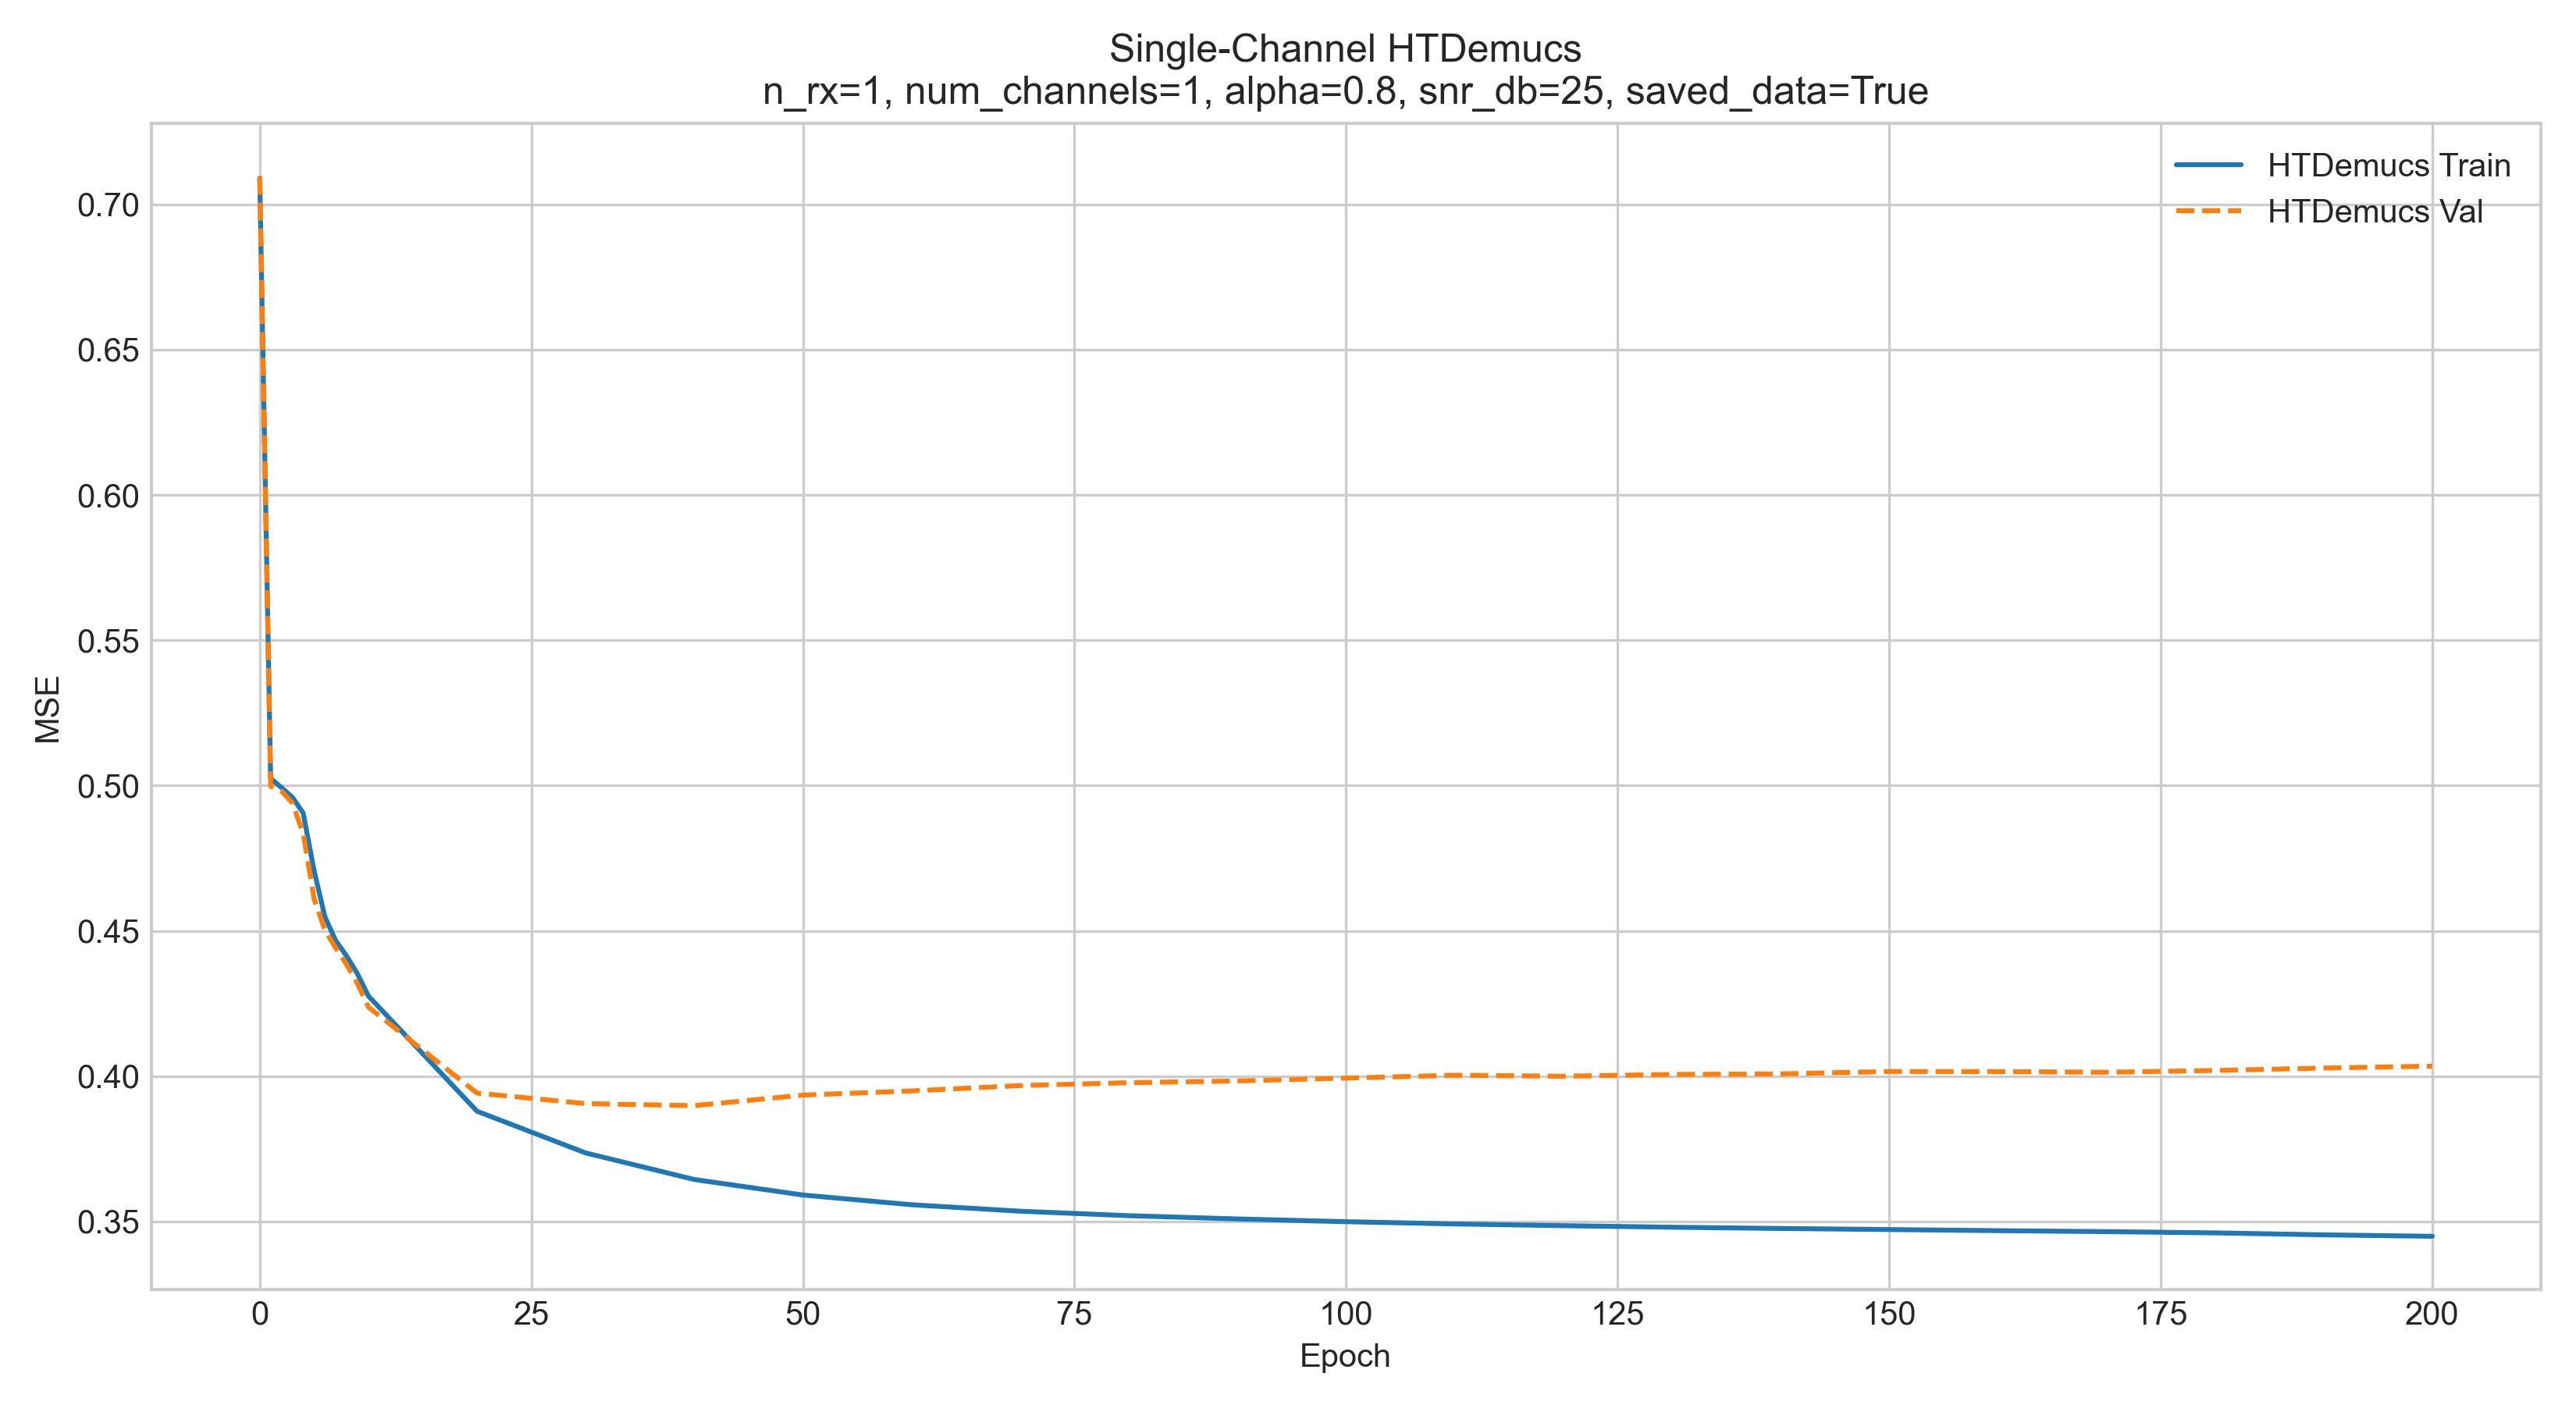
\includegraphics[width=0.95\columnwidth]{figures/htdemucs_train_val.png}
    \caption{Single-channel HTDemucs training and validation curves. Compared with Hybrid, LSTM, and IQ\_CNN, HTDemucs improved much more slowly and did not catch up within the same short budget.}
    \label{fig:demucs_train}
\end{figure}

\section{Experiments}
This report details the experiments that were preformed for the single channel separation problem, the two channel separation problem and the four channel separation problem. The number of channels represents the number of antennas that are receiving the transmitted data. Because each antenna will get the data at a different time phase the more channels added the more difficult the problem becomes.

\subsection{Single-Channel Separation Problem}
The single-channel experiments used the current good configuration: one receive channel ($n_{rx}=1$ and \texttt{num\_channels}=1), saved fixed data rather than on-the-fly generation, no additive noise in the baseline comparison, and a reference interference strength of $\alpha=0.8$. Under this setup, Hybrid, LSTM, and IQ\_CNN all reached essentially perfect symbol recovery and very low waveform error, while HTDemucs improved more slowly and remained far behind the other learned models within the same short training budget. Because symbol accuracy saturated for the strongest three models, waveform MSE was the most useful discriminative metric in the reference comparison shown in Table~\ref{tab:singlechannel} and Fig.~\ref{fig:single_wave}.

\begin{table}[htbp]
\centering
\caption{Single-channel reference comparison at the current good baseline configuration.}
\label{tab:singlechannel}
\begin{tabular}{lccc}
\toprule
Model & Wave MSE & SDR (dB) & Symbol Acc \\
\midrule
LSTM & 0.000008 & 47.70 & 1.000 \\
IQ\_CNN & 0.000029 & 42.49 & 1.000 \\
Hybrid & 0.000081 & 37.90 & 1.000 \\
HTDemucs & 0.428018 & 0.68 & 0.397 \\
\bottomrule
\end{tabular}
\end{table}

\begin{figure}[htbp]
    \centering
    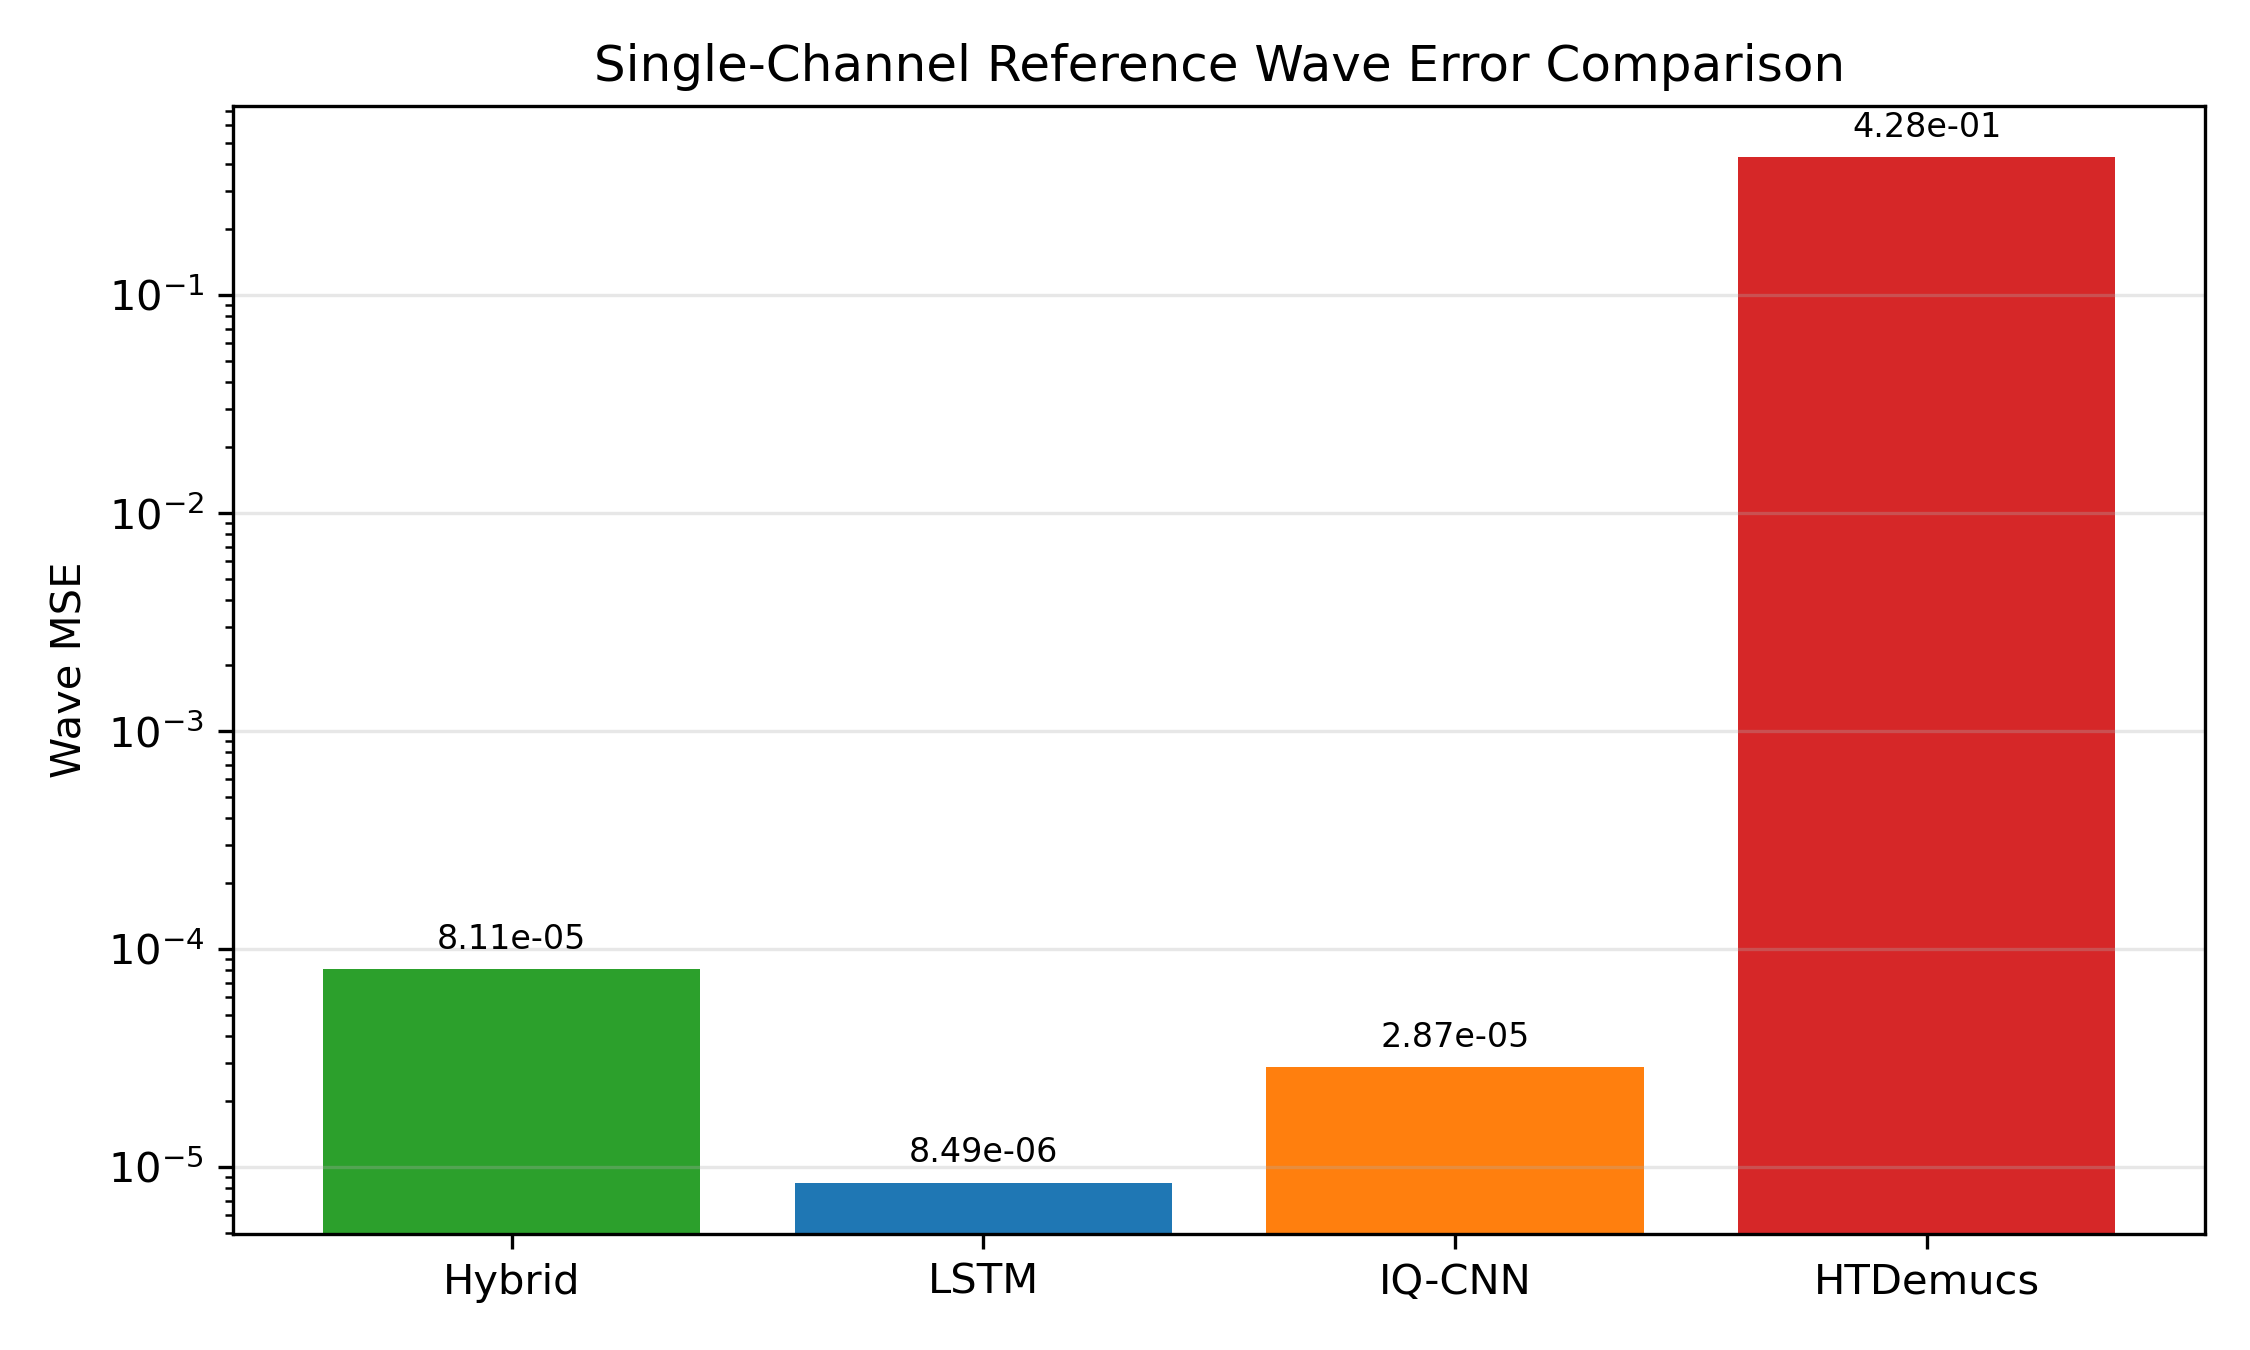
\includegraphics[width=0.95\columnwidth]{figures/single_channel_reference_wave_comparison.png}
    \caption{Single-channel reference waveform comparison. Since Hybrid, LSTM, and IQ\_CNN all saturated symbol accuracy, waveform error was the main metric used to separate them.}
    \label{fig:single_wave}
\end{figure}

The alpha sweep was the most revealing single-channel experiment. Moving from the good baseline at $\alpha=0.8$ toward equal-strength interference caused a sharp increase in error near $\alpha=1.0$. Hybrid, LSTM, and IQ\_CNN all performed well at $\alpha=0.80$ and $\alpha=0.95$, but the equal-strength point produced a clear failure band: by $\alpha=1.0$, all three models collapsed to roughly $0.25$ validation MSE and symbol accuracy near $57\%$. The effect was not monotone. Performance improved again after moving away from the symmetric point, and by $\alpha=1.05$ the learned models had recovered to near-perfect symbol accuracy. This indicates that the hardest single-channel case is the symmetric mixture itself. When the SOI and interferer have almost identical strength, the problem becomes much less identifiable under plain MSE training, so the separator stalls near the well-known $\approx 0.25$ error floor.

\begin{table}[htbp]
\centering
\caption{Selected points from the single-channel alpha sweep.}
\label{tab:alphaselected}
\begin{tabular}{lccc}
\toprule
$\alpha$ & Hybrid MSE & LSTM MSE & IQ\_CNN MSE \\
\midrule
0.80 & 0.000165 & 0.000019 & 0.000040 \\
0.98 & 0.000797 & 0.000696 & 0.125624 \\
1.00 & 0.249567 & 0.249504 & 0.249526 \\
1.02 & 0.089617 & 0.000605 & 0.022320 \\
1.05 & 0.000143 & 0.000085 & 0.000154 \\
\bottomrule
\end{tabular}
\end{table}

\begin{figure}[htbp]
    \centering
    \begin{subfigure}{0.48\columnwidth}
        \centering
        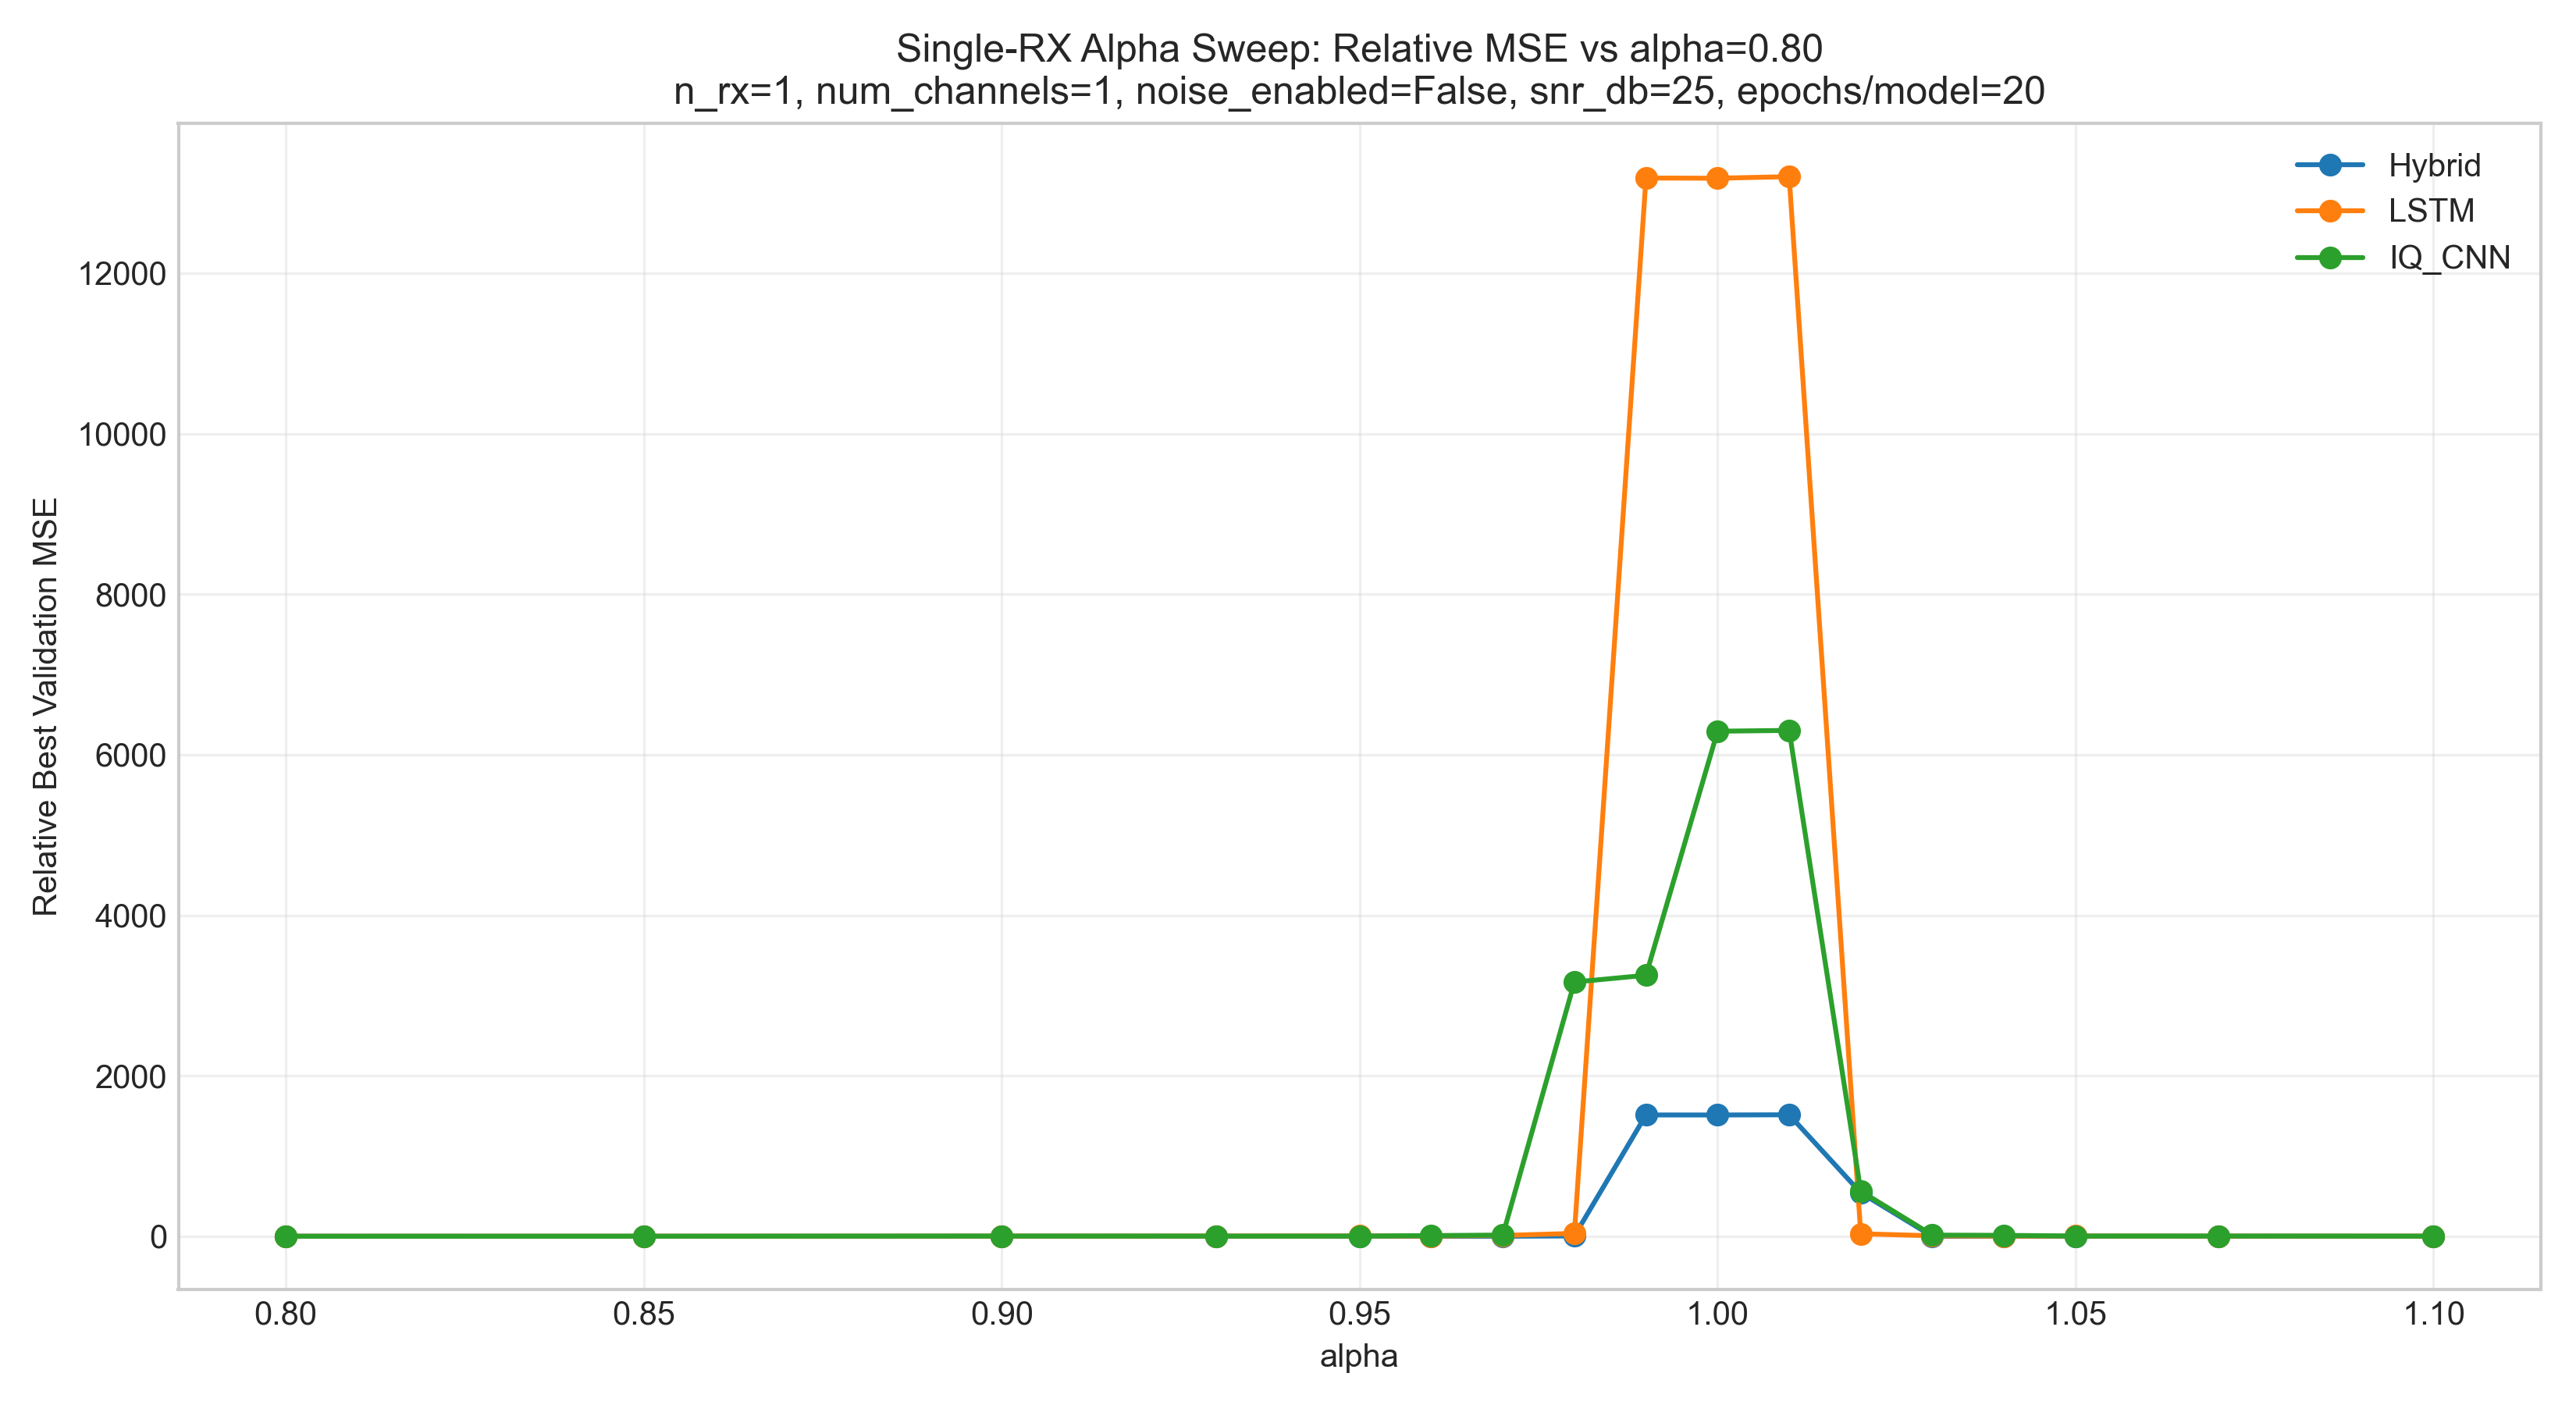
\includegraphics[width=\linewidth]{figures/alpha_vs_relative_mse.png}
        \caption{Relative wave MSE vs. $\alpha$}
    \end{subfigure}
    \hfill
    \begin{subfigure}{0.48\columnwidth}
        \centering
        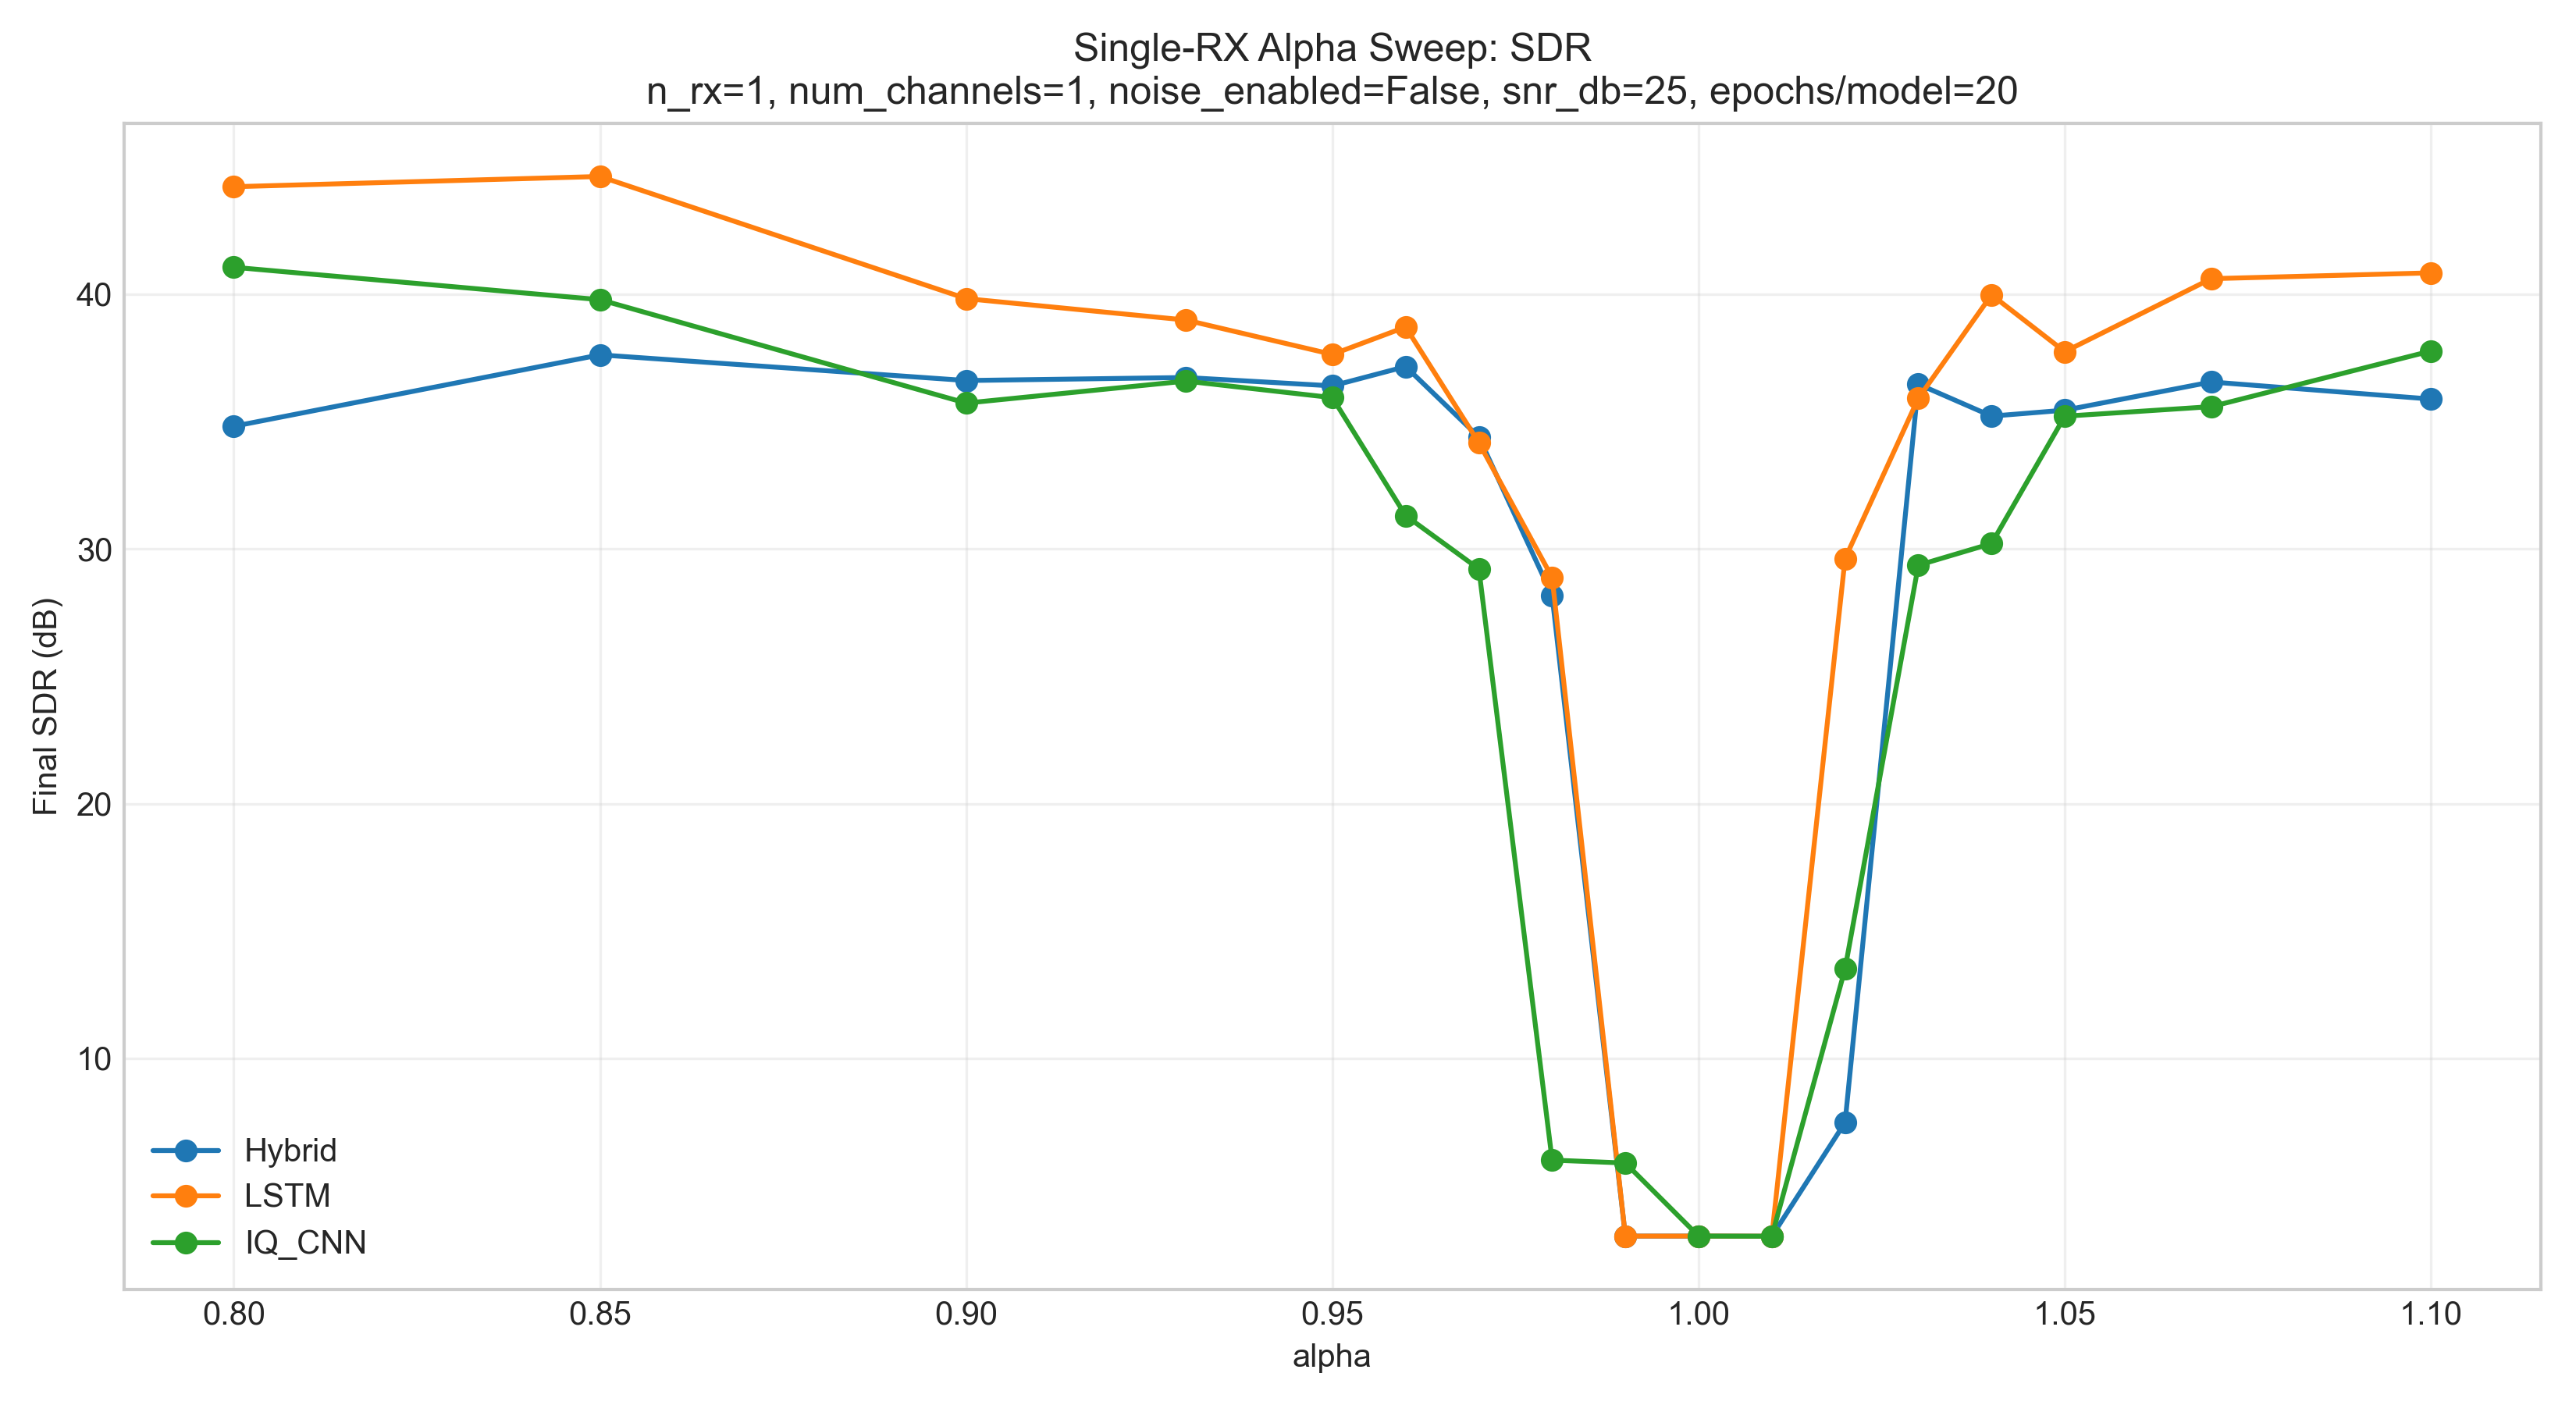
\includegraphics[width=\linewidth]{figures/alpha_vs_sdr_db.png}
        \caption{SDR vs. $\alpha$}
    \end{subfigure}
    \caption{Single-channel alpha sweep. The error peak at $\alpha\approx1.0$ shows that the hardest point is the equal-strength mixture, not simply the largest interference scale.}
    \label{fig:alpha_summary}
\end{figure}

\begin{figure}[htbp]
    \centering
    \begin{subfigure}{0.48\columnwidth}
        \centering
        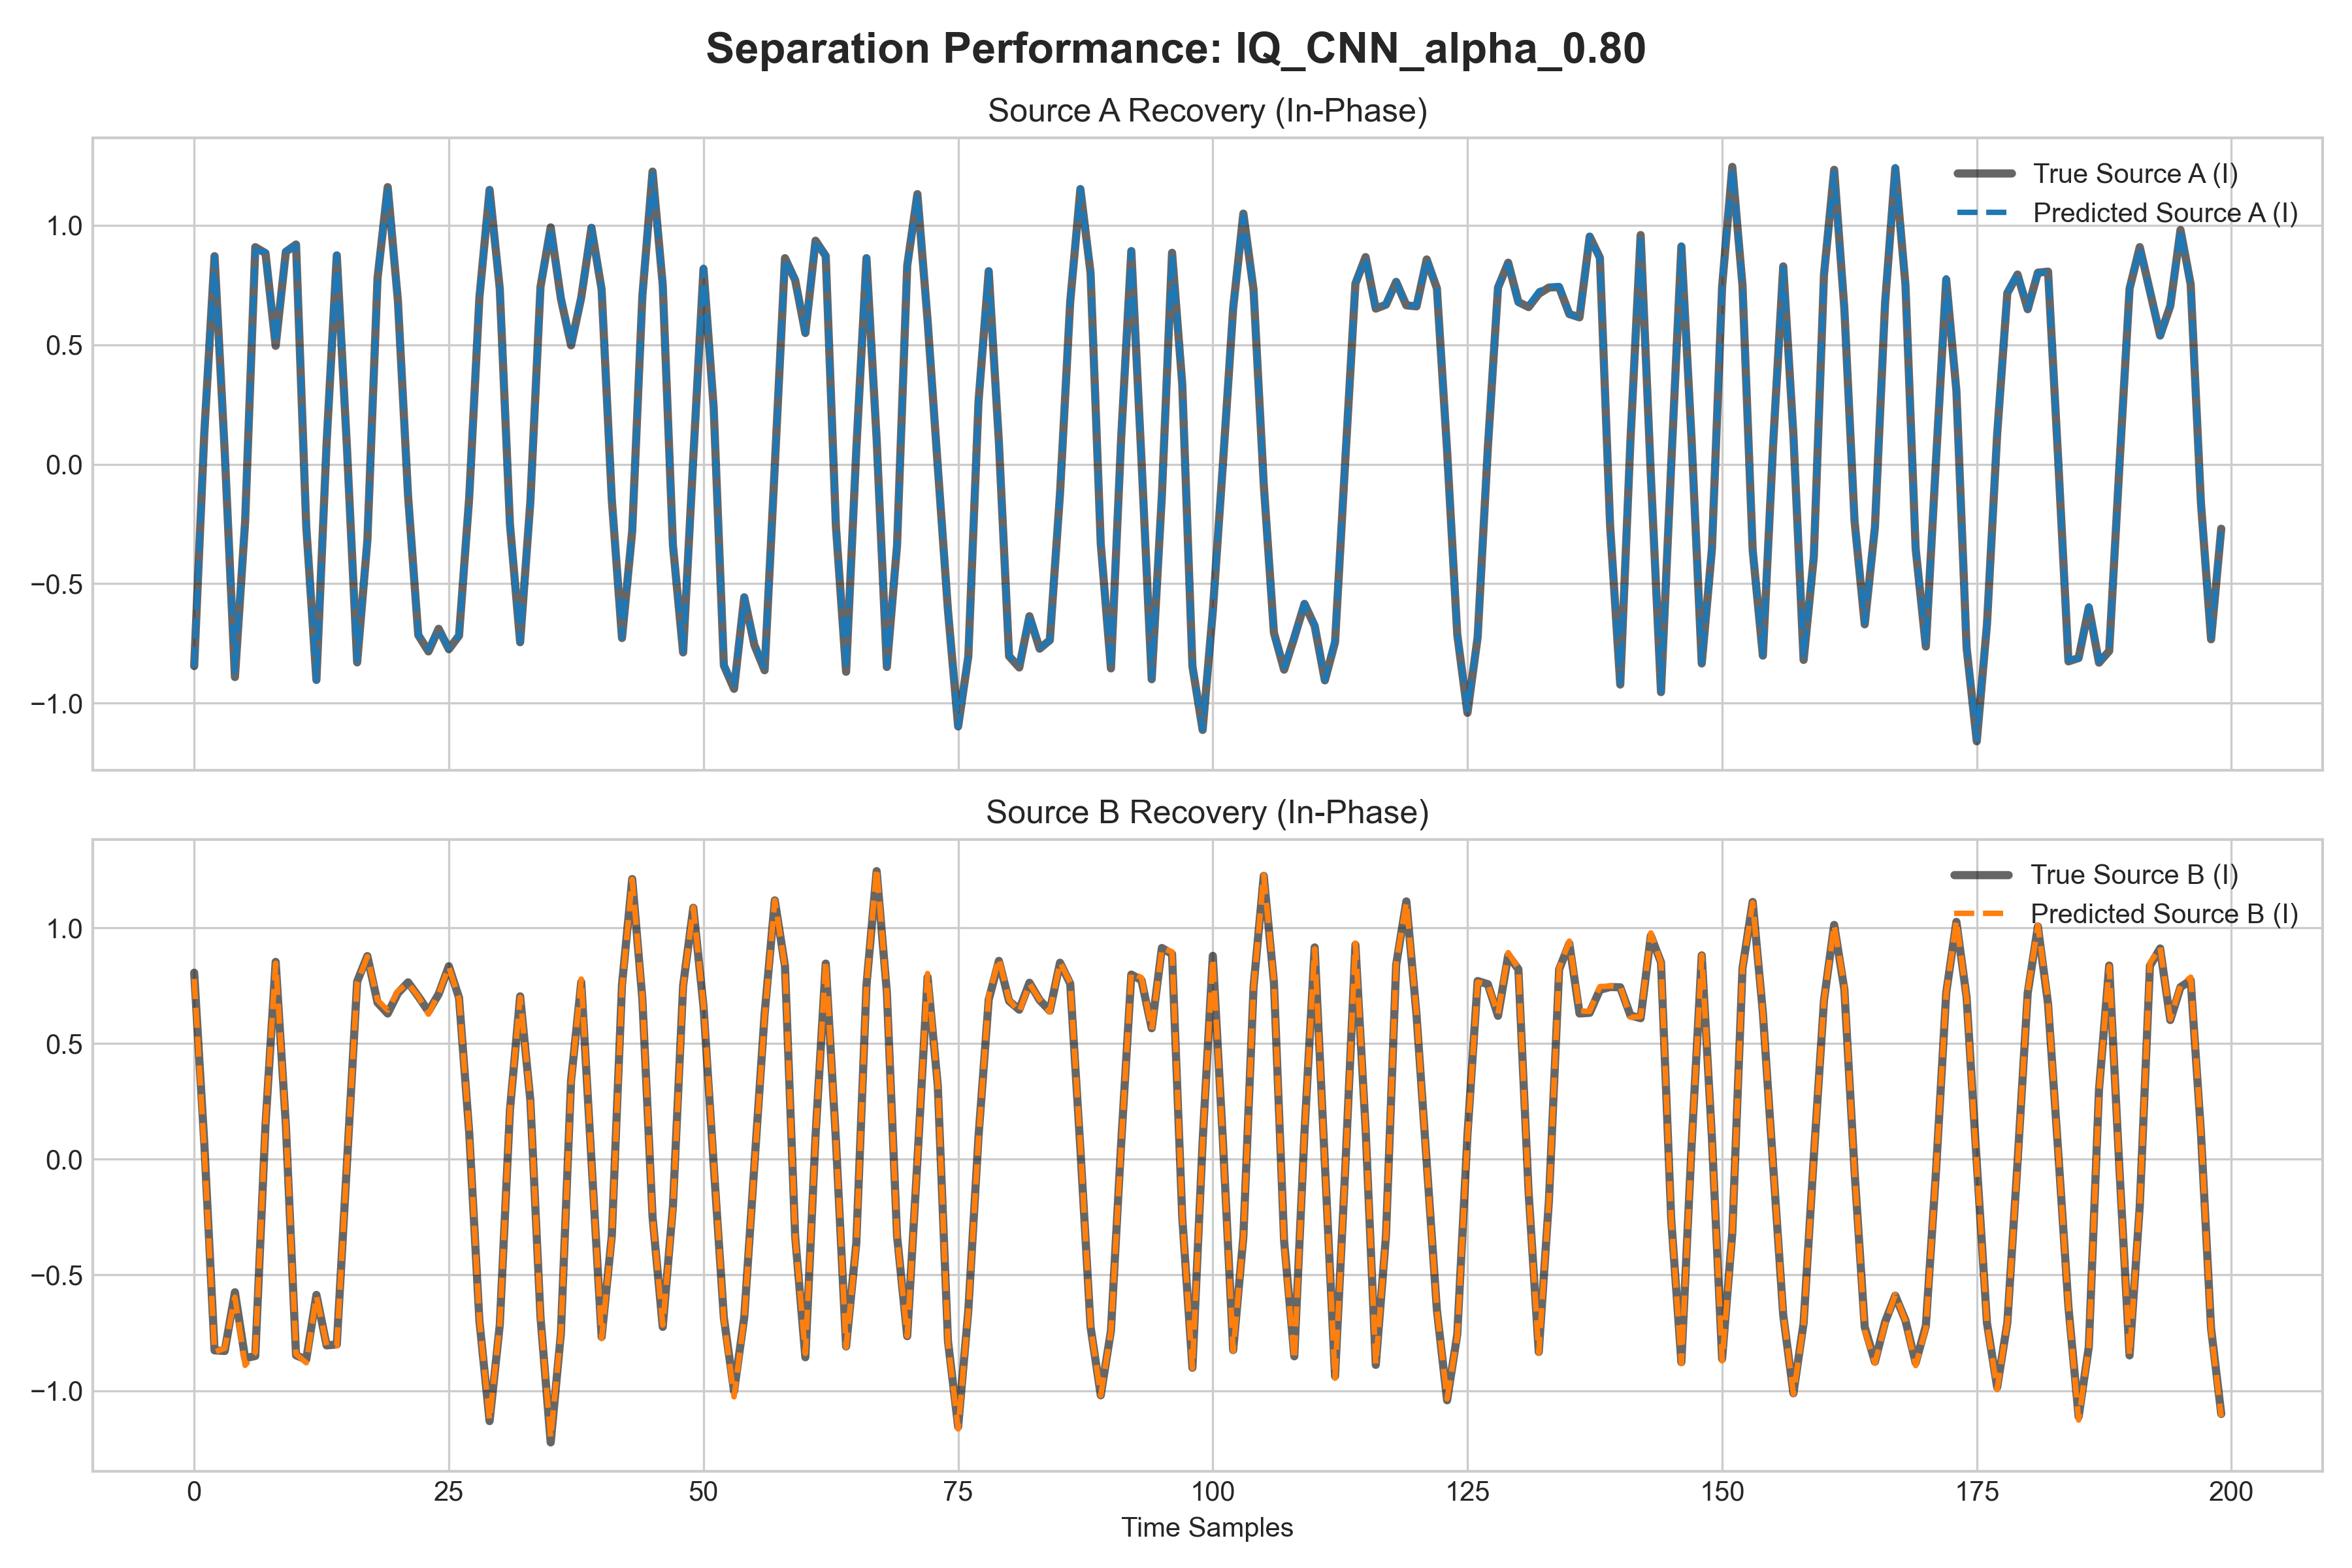
\includegraphics[width=\linewidth]{figures/IQ_CNN_alpha_0p80_separation.png}
        \caption{IQ\_CNN at $\alpha=0.80$}
    \end{subfigure}
    \hfill
    \begin{subfigure}{0.48\columnwidth}
        \centering
        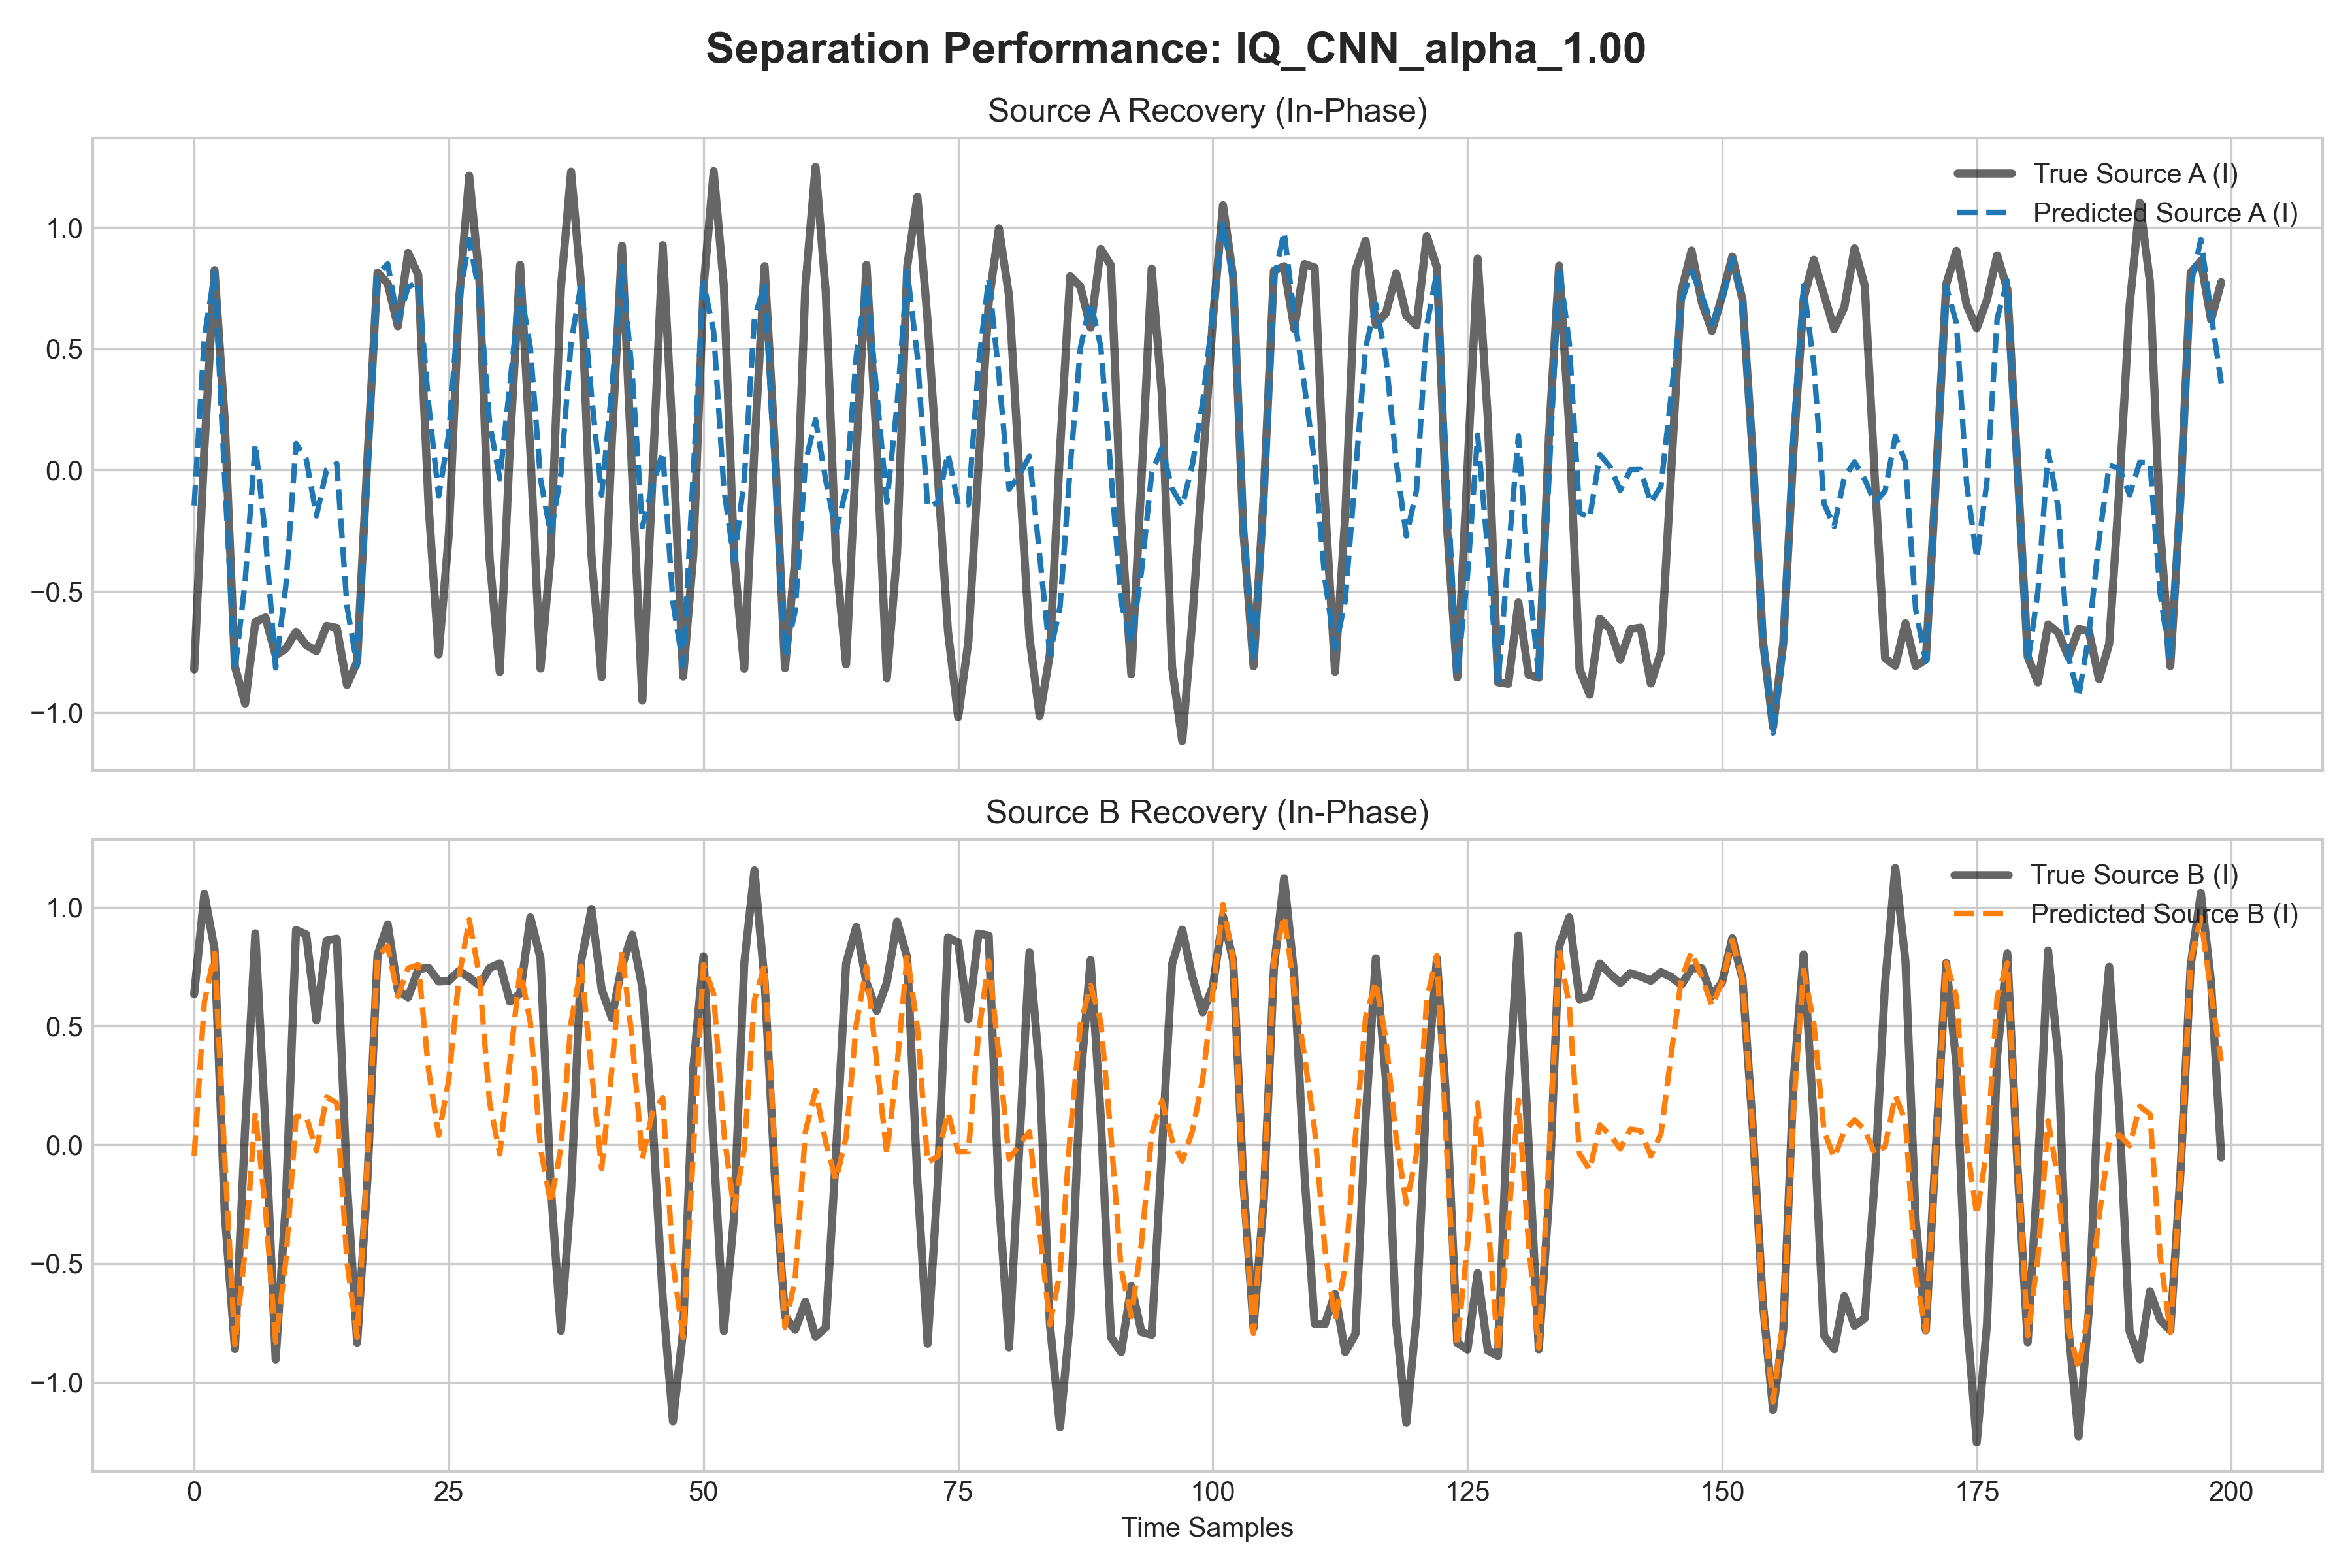
\includegraphics[width=\linewidth]{figures/IQ_CNN_alpha_1p00_separation.png}
        \caption{IQ\_CNN at $\alpha=1.00$}
    \end{subfigure}
    \caption{Waveform recovery at the good point and the failure point for the same model. The degradation at $\alpha=1.00$ is visually obvious even before looking at the summary metrics.}
    \label{fig:alpha_examples}
\end{figure}

The noise sweep showed a different pattern. Holding $\alpha=0.8$ fixed and increasing Gaussian noise variance caused a gradual, monotone rise in waveform error and a matching decline in symbol accuracy. For the completed sweep points through variance $0.12$, best validation MSE rose from near-zero at variance $0.0$ to roughly $0.145$, while symbol accuracy decreased from $1.0$ to about $0.80$ for all three learned models. Unlike the alpha sweep, the noise sweep did not show a sharp symmetry-driven failure band; instead, it degraded performance smoothly as the variance increased.

\begin{figure}[htbp]
    \centering
    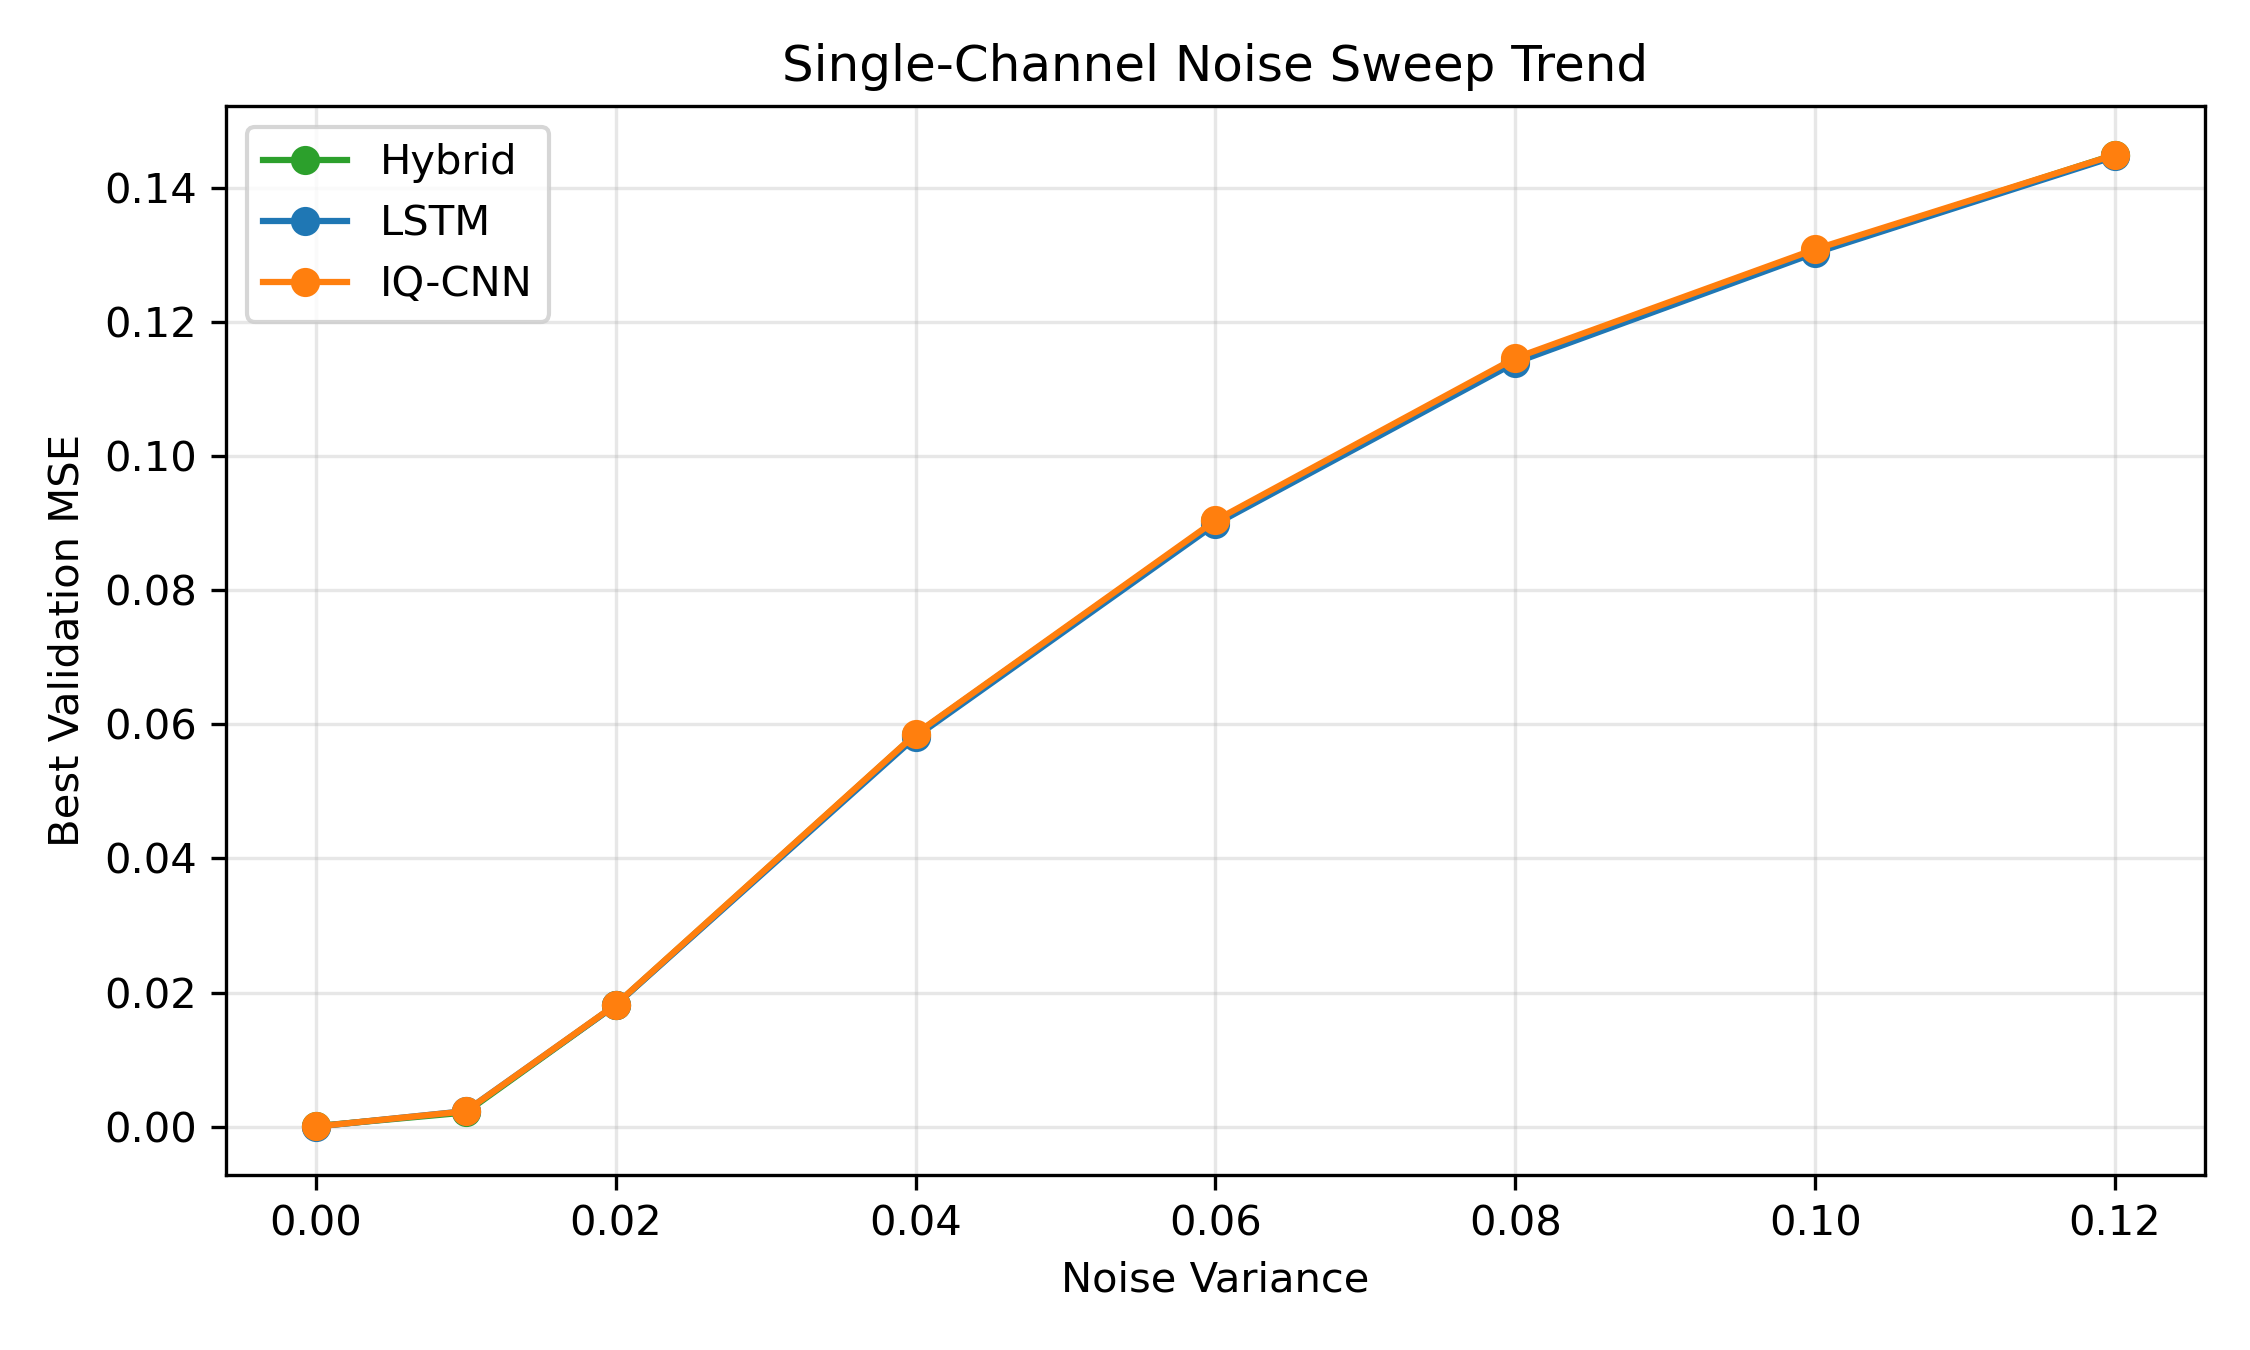
\includegraphics[width=0.95\columnwidth]{figures/noise_variance_vs_best_val_mse_current.png}
    \caption{Current noise-sweep trend for the completed variance points. The rise in waveform error is gradual rather than abrupt.}
    \label{fig:noise_current}
\end{figure}

\subsection{2-Channel Separation Problem}
The second major experiment moved to two receive channels. This step was especially important for evaluating FastICA fairly, because ICA is fundamentally a multivariate blind source separation method and benefits from multiple observations. A preliminary validation step compared FastICA in the one-channel and two-channel settings. Moving from one complex receive channel to two receive channels improved FastICA dramatically: wave MSE decreased from $0.3824$ to $0.0660$, SDR increased from $1.17$ dB to $10.76$ dB, and symbol accuracy improved from about 40\% to approximately 97.3\% for both the SOI and the interference.

After establishing that FastICA needed two receive channels to act as a fairer baseline, we compared FastICA against the learned models on the same fixed two-channel dataset generated through the main project generator. In this reference comparison, FastICA remained the weakest method by a large margin in waveform quality, while the learned models clustered more closely together. LSTM produced the highest symbol accuracy among the learned models, but the gap between the learned models was small. In contrast, FastICA's wave MSE remained much higher than all learned models. This result supports the view that a multichannel FastICA baseline is much fairer than the single-channel baseline, but still not competitive with the learned separators in waveform recovery.

\begin{figure}[htbp]
    \centering
    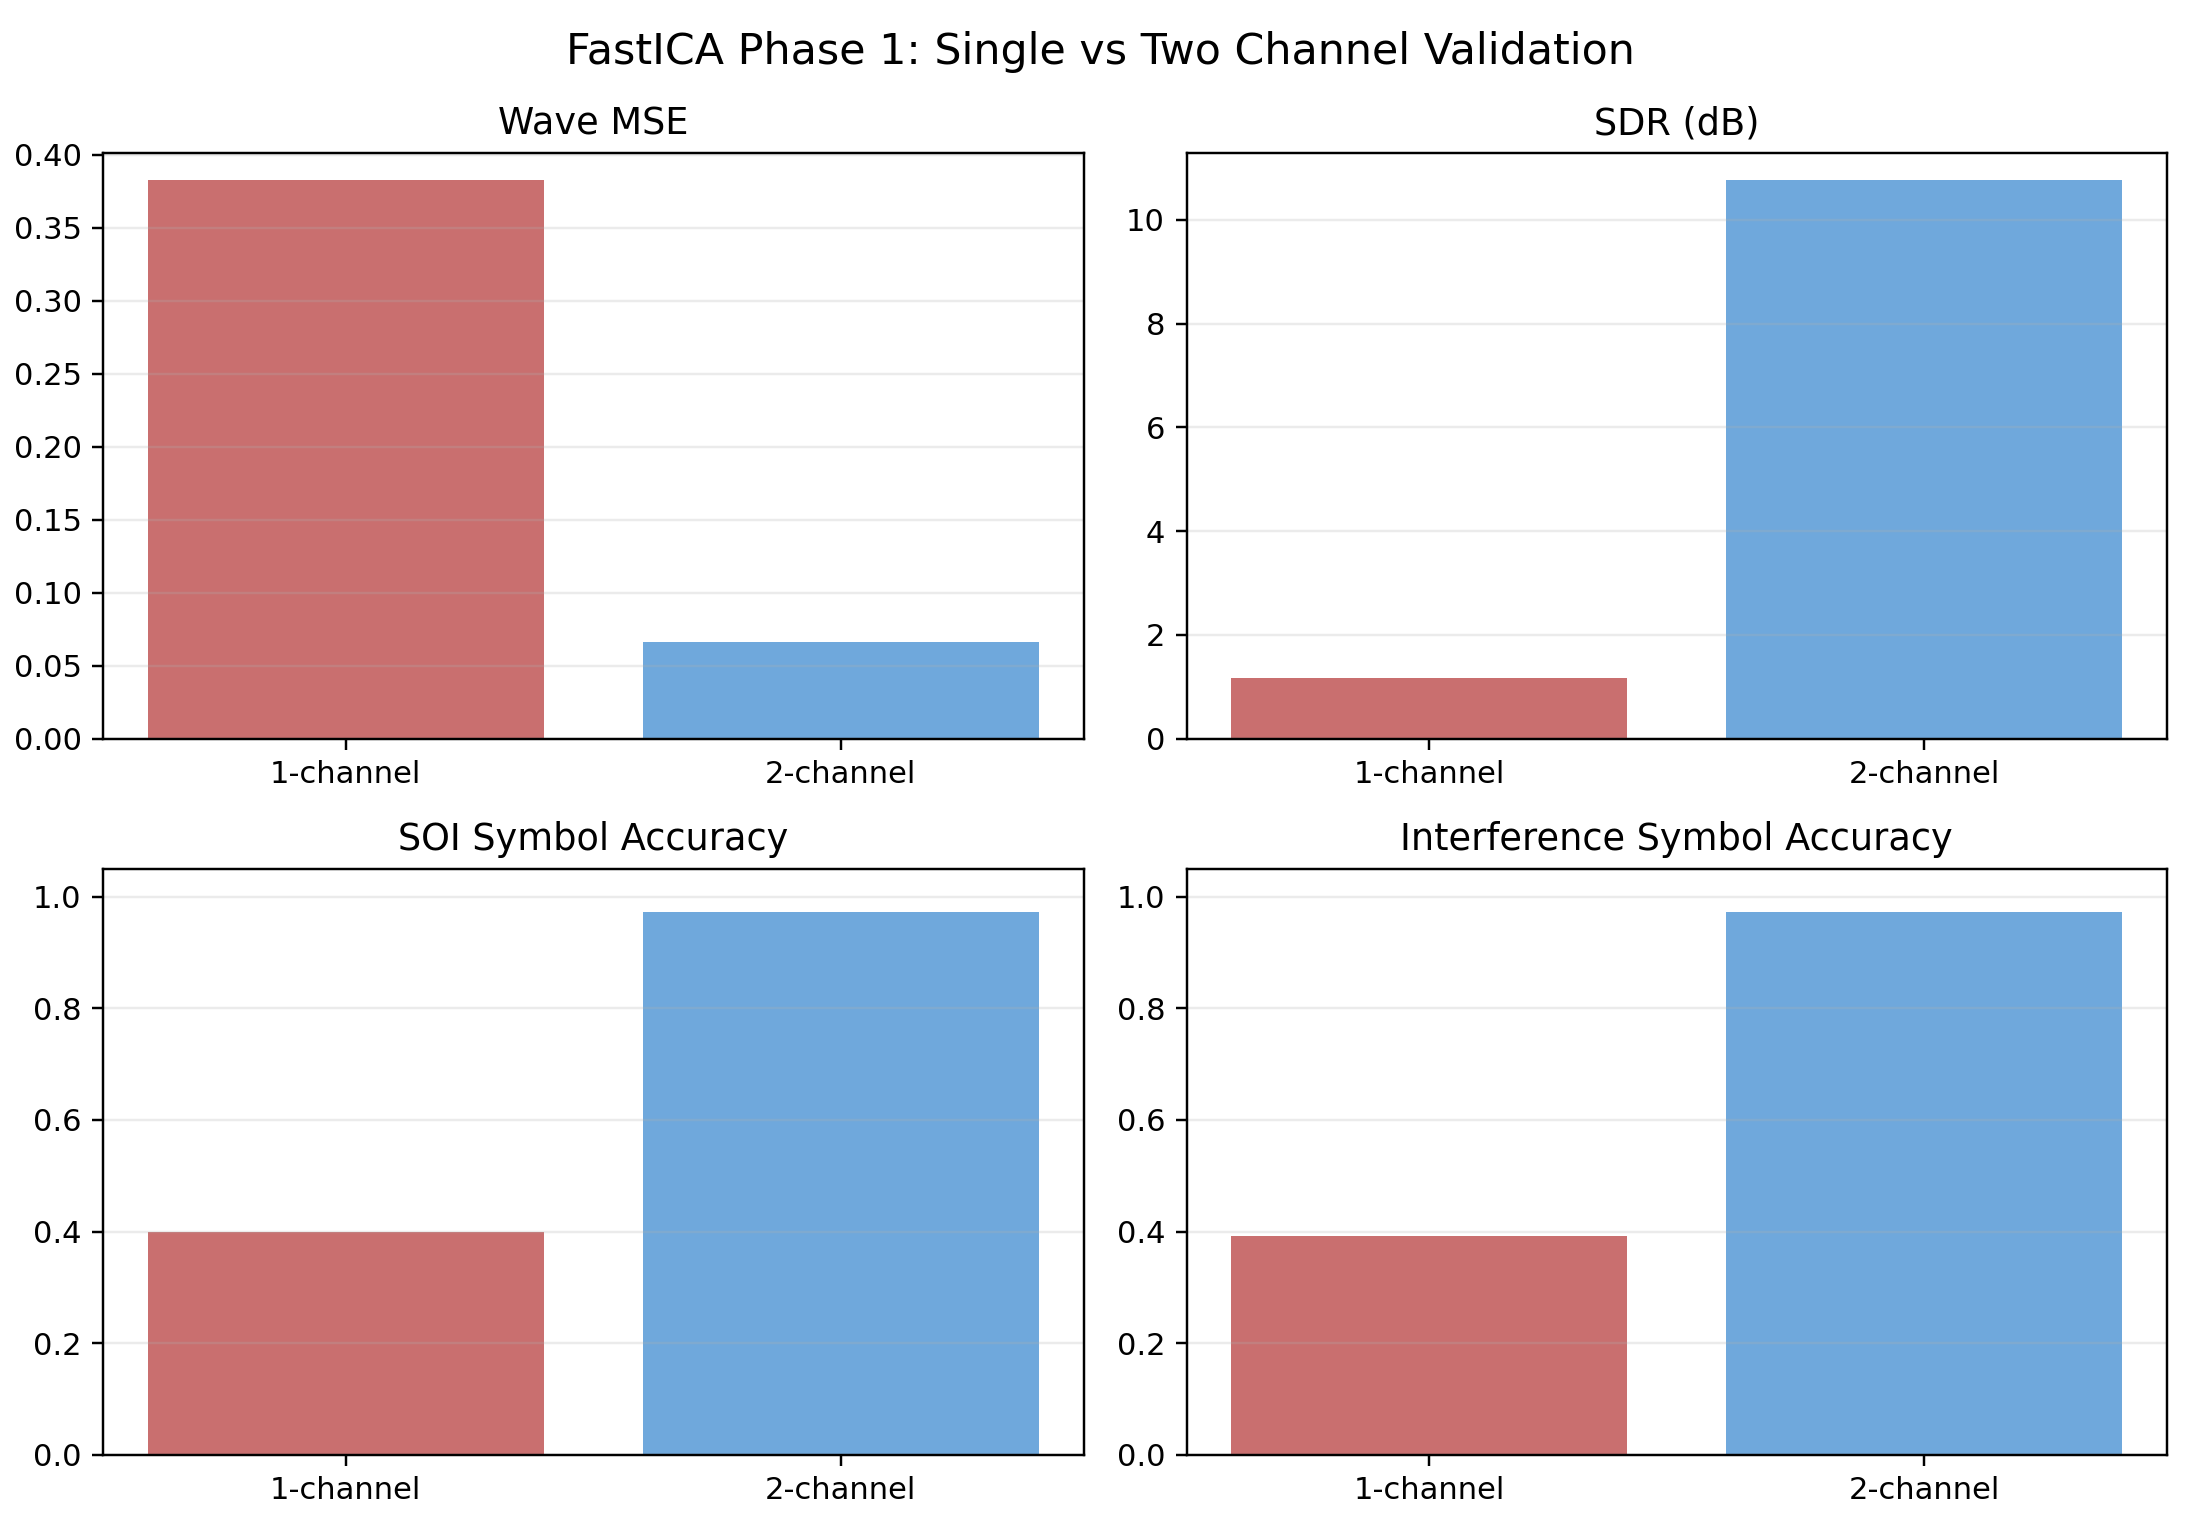
\includegraphics[width=0.95\columnwidth]{figures/fastica_phase1_comparison.png}
    \caption{FastICA Phase 1 validation: moving from one receive channel to two receive channels greatly improves the baseline. This confirms that ICA should not be treated as a meaningful one-channel baseline for the current problem.}
    \label{fig:fastica_phase1}
\end{figure}

\subsection{4-Channel Separation Problem}
For the four channel separation problem a simple Mean Squared Error (MSE) loss was optimized using Adam \cite{adam_optimization}. All models were trained on $10,000$ training examples and validated on $1,000$ testing examples. The training for each model ran for $300$ epochs and used the learning rate, batch size, and architecture settings selected during the earlier tuning stage. The experiments showed that when moving up to the problem of four receive channels none of the created models were able to generalize to the validation set. Fiugre \ref{fig:validation_mse}. The longer the models trained the more they overfit to the training data. \textcolor{blue}{Once Hyrum has experiments for single channel and two channel we can fill this section in}
\begin{figure}[htbp]
    \centering
    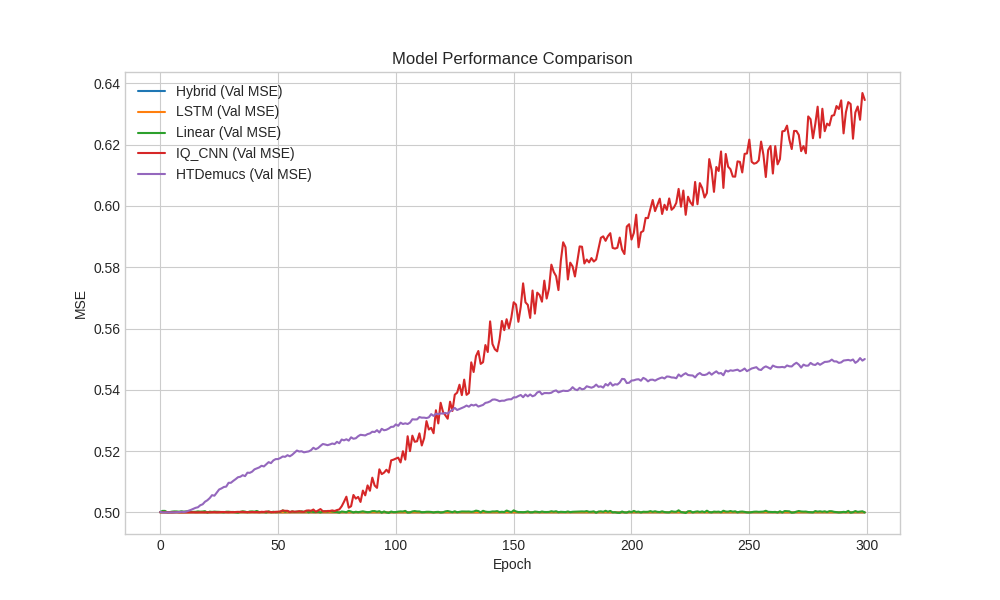
\includegraphics[width=1\linewidth]{validation mse.png}
    \caption{Validation MSE For All Models After 300 Epochs}
    \label{fig:validation_mse}
\end{figure}

\section{Conclusion}
This work produced four main lessons. First, in the current single-channel configuration, Hybrid, LSTM, and IQ\_CNN all learned the separation problem reliably and reached near-perfect symbol recovery, while HTDemucs learned much more slowly and remained less competitive within the same short budget. Second, FastICA is not a meaningful one-channel baseline for the current problem, but it becomes substantially fairer when given two receive channels. Third, the single-channel alpha sweep showed that the most difficult case is the equal-strength mixture near $\alpha=1.0$, where plain MSE training encounters a symmetry-driven failure band. Finally, the noise sweep showed a different failure mode: increasing Gaussian noise variance degraded waveform recovery and symbol accuracy gradually rather than abruptly. Together, these results show that waveform error and symbol recovery do not fail in the same way, and both are needed to fully understand RF source-separation behavior.

\newpage

\bibliographystyle{IEEEtran}
\bibliography{references/references}

\appendices

\section{Music Source Separation}
At the start of the semester our sponsor tasked us with Music Source Separation (MSS). Music source separation has evolved rapidly with the introduction of deep learning. Early methods relied on non-negative matrix factorization and handcrafted features, which were limited in their ability to disentangle overlapping sources.
MSS takes as input a song and attempts to isolate specific parts of that song. The most common dataset used in the field is MUSDB18. This dataset contains 150 full length music tracks as well as their isolated parts. MUSDB18 contains isolated drums, bass, voice, and an other category for everything else. The sponsor recommended that we use the D3Net architecture \cite{d3net}. D3Net (Dense Dilated Deep Neural Network) is a convolutional encoder–decoder architecture that combines dilated convolutions, dense skip connections, and multi-scale feature extraction \cite{d3net}. It was proposed as a state-of-the-art solution for music source separation by effectively capturing both local spectral patterns and long-range temporal context. This architecture did significantly better than the ones before and acts as a good baseline. Significant time was spent understanding and starting to implement this architecture.

After some time a literature review was completed that showed that the recommended D3Net was far behind the state of the art in MSS.
\begin{figure}[H]
    \centering
    \includegraphics[width=0.95\columnwidth]{figures/musdb18_model_comparisons.png}
    \caption{The figure above shows the current leaderboard for MSS accuracy on a variety of models. The figure was pulled from \cite{musdb18_model_comparison}} https://opencodepapers-b7572d.gitlab.io/benchmarks/music-source-separation-on-musdb18.html
    \label{fig:placeholder_frequency}
\end{figure}

This realization led the team to Demucs \ref{fig:Demucs Architecture} (The top preforming architecture on MSS). This architecture was successfully leveraged to solve the problem of MSS to a level that the sponsor was satisfied with. It included a user interface and a command line interface that allowed the user to configure things to their liking.

Noticing how successful this architecture was in MSS the team decided that it would be a good idea to try it on RF separation. Although the MSS problem was not the final problem the team ended with, it acted as a stepping stone in understanding the future problems the team tackled.

\section{MIT Interference Challenge}
\textcolor{blue}{This section will be updated before the final report}

\end{document}
